\documentclass[12pt,bibliography=oldstyle,DIV=12,parskip=half-]{scrreprt}
\newif\iflatexml\latexmlfalse
\usepackage{xstring}
\newcommand{\includePrueba}[1]{\input{#1}}
\newcommand{\includeFileOrFigure}[1]{%
  \IfBeginWith{#1}{figures/}{%
    \begin{figure}[H]
      \figureStyle
      \StrBefore[2]{#1}{/}[\temp]
      \tikzsetnextfilename{figures/femigracion/femigracion}
\begin{tikzpicture}[
    font=\footnotesize,
    thick
  ]
\usetikzlibrary{positioning,fit,calc,shapes}
\def\nw{1cm}

\makeatletter
\pgfkeys{/pgf/.cd,
  parallelepiped offset x/.initial=2mm,
  parallelepiped offset y/.initial=2mm
}
\pgfdeclareshape{parallelepiped}
{
  \inheritsavedanchors[from=rectangle] % this is nearly a rectangle
  \inheritanchorborder[from=rectangle]
  \inheritanchor[from=rectangle]{north}
  \inheritanchor[from=rectangle]{north west}
  \inheritanchor[from=rectangle]{north east}
  \inheritanchor[from=rectangle]{center}
  \inheritanchor[from=rectangle]{west}
  \inheritanchor[from=rectangle]{east}
  \inheritanchor[from=rectangle]{mid}
  \inheritanchor[from=rectangle]{mid west}
  \inheritanchor[from=rectangle]{mid east}
  \inheritanchor[from=rectangle]{base}
  \inheritanchor[from=rectangle]{base west}
  \inheritanchor[from=rectangle]{base east}
  \inheritanchor[from=rectangle]{south}
  \inheritanchor[from=rectangle]{south west}
  \inheritanchor[from=rectangle]{south east}
  \backgroundpath{
    % store lower right in xa/ya and upper right in xb/yb
    \southwest \pgf@xa=\pgf@x \pgf@ya=\pgf@y
    \northeast \pgf@xb=\pgf@x \pgf@yb=\pgf@y
    \pgfmathsetlength\pgfutil@tempdima{\pgfkeysvalueof{/pgf/parallelepiped offset x}}
    \pgfmathsetlength\pgfutil@tempdimb{\pgfkeysvalueof{/pgf/parallelepiped offset y}}
    \def\ppd@offset{\pgfpoint{\pgfutil@tempdima}{\pgfutil@tempdimb}}
    \pgfpathmoveto{\pgfqpoint{\pgf@xa}{\pgf@ya}}
    \pgfpathlineto{\pgfqpoint{\pgf@xb}{\pgf@ya}}
    \pgfpathlineto{\pgfqpoint{\pgf@xb}{\pgf@yb}}
    \pgfpathlineto{\pgfqpoint{\pgf@xa}{\pgf@yb}}
    \pgfpathclose
    \pgfpathmoveto{\pgfqpoint{\pgf@xb}{\pgf@ya}}
    \pgfpathlineto{\pgfpointadd{\pgfpoint{\pgf@xb}{\pgf@ya}}{\ppd@offset}}
    \pgfpathlineto{\pgfpointadd{\pgfpoint{\pgf@xb}{\pgf@yb}}{\ppd@offset}}
    \pgfpathlineto{\pgfpointadd{\pgfpoint{\pgf@xa}{\pgf@yb}}{\ppd@offset}}
    \pgfpathlineto{\pgfqpoint{\pgf@xa}{\pgf@yb}}
    \pgfpathmoveto{\pgfqpoint{\pgf@xb}{\pgf@yb}}
    \pgfpathlineto{\pgfpointadd{\pgfpoint{\pgf@xb}{\pgf@yb}}{\ppd@offset}}
  }
}
\makeatother


\node[cloud,cloud ignores aspect,draw,,minimum width=1.5*\nw,minimum height=\nw] (internet) {Internet};
\node[parallelepiped,draw,minimum width=\nw,minimum height=.75*\nw,node distance=.6*\nw,below = of internet] (firewall) {Firewall};
\node[arrow box,draw=green,arrow box shaft width=.25*\nw,node distance=.6*\nw,below = of firewall] (frontend) {};
\node[arrow box,draw=blue,arrow box shaft width=.25*\nw,node distance=.6*\nw,right = of frontend] (redir) {};
\node[chamfered rectangle,chamfered rectangle corners=north west,draw=magenta,node distance=2*\nw,minimum width=.6*\nw,minimum height=.6*\nw,right = of redir] (svn) {SVN};
\coordinate (aux) at ($ (redir.south) - (0,.6*\nw) $);
\coordinate (auxfe) at ($ (frontend.south) - (0,.6*\nw) $);

% \tikzstyle{srv}=[cylinder,shape border rotate=90, shape aspect=0.4,minimum height=1.2*\nw,minimum width=0.8*\nw,node distance=.5*\nw]
\tikzstyle{srv}=[minimum height=1.4*\nw,minimum width=0.9*\nw,node distance=0.4*\nw]
\tikzstyle{blue}=[draw=blue]
\tikzstyle{green}=[draw=green]
\tikzstyle{magenta}=[draw=magenta]
\node[blue,srv,node distance=.6*\nw, below = of aux,xshift=-.4*\nw ] (srv1) {srv};
\node[green,srv, below left = of srv1 ] (srv2) {srv};
\node[blue,srv, below right = of srv1 ] (srv3) {srv};
\node[green,srv, above left = of srv2 ] (srv4) {srv};
\node[blue,srv, above right = of srv3 ] (srv5) {srv};
\node[blue,srv, below right = of srv5 ] (srv6) {srv};

\draw[-,blue] (srv1.north)  |- (aux) -- (redir.south);
\draw[-,blue] (srv2.north) |- (aux) -- (redir.south);
\draw[-,blue] (srv3.north) |- (aux) -- (redir.south);
\draw[-,blue] (srv4.north) |- (aux) -- (redir.south);
\draw[-,blue] (srv5.north) |- (aux) -- (redir.south);
\draw[-,blue] (srv6.north) |- (aux) -- (redir.south);
\draw[-,green] (srv2.north) |- (auxfe) -- (frontend.south);
\draw[-,green] (srv4.north) |- (auxfe) -- (frontend.south);

\draw[-,dashed,draw=magenta] (svn.west)  -- (redir.east);
\draw[-] (frontend.north)  -- (firewall.south);
\draw[-,green] (frontend.east)  -- (redir.west);
\draw[-] (firewall.north)  -- (internet.south);

\tikzstyle{agent}=[circle,magenta,minimum height=.3*\nw,minimum width=.3*\nw,inner sep=0mm];
%\node[agent] at ($ (srv1.south east) + (-.25*\nw,.25*\nw) $) (c1) {C};
\node[agent] at ($ (srv2.south east) + (-.25*\nw,.25*\nw) $) (c2) {C};
%\node[agent] at ($ (srv3.south east) + (-.25*\nw,.25*\nw) $) (c3) {C};
\node[agent] at ($ (srv4.south east) + (-.25*\nw,.25*\nw) $) (c4) {C};
%\node[agent] at ($ (srv5.south east) + (-.25*\nw,.25*\nw) $) (c5) {C};
%\node[agent] at ($ (srv6.south east) + (-.25*\nw,.25*\nw) $) (c6) {C};

\tikzstyle{consul}=[circle,magenta,node distance=.5*\nw,minimum height=.6*\nw,minimum width=.6*\nw,inner sep=0mm];
\node[consul, node distance=1*\nw, left=of srv4]  (consul1) {C};
\node[consul, above=of consul1]  (consul2) {C};
\node[consul, above=of consul2]  (consul3) {C};
\node[consul, above=of consul3]  (consul4) {C};
\node[consul, above=of consul4]  (consul5) {C};

\coordinate (aux1) at ($ (srv4.south) - (0,2.2*\nw) $);
\coordinate (aux2) at ($ (consul2.east) + (0.2*\nw,0) $);
\coordinate (aux3) at ($ (consul3.west) - (0.2*\nw,0) $);

\draw[-,dashed,magenta] (c4.south)  |- (aux1) -| (consul1.south);
%\draw[-,dashed] (c3.south)  |- (aux1) -| (consul1.south);
\draw[-,dashed,magenta] (c2.south)  |- (aux1) -| (aux3) -- (consul3.west);
%\draw[-,dashed] (c1.south)  |- (aux1);
%\draw[-,dashed] (c5.south)  |- (aux1);
%\draw[-,dashed] (c6.south)  |- (aux1);
\draw[-,dashed,magenta] (consul1.north)  -- (consul2.south);
\draw[-,dashed,magenta] (consul2.north)  -- (consul3.south);
\draw[-,dashed,magenta] (consul3.north)  -- (consul4.south);
\draw[-,dashed,magenta] (consul4.north)  -- (consul5.south);

\coordinate (aux4) at ($ (frontend.west) - (\nw,0) $);
\draw[-,dashed,magenta] (consul4.east)  -| (aux4) -- (frontend.west);

\end{tikzpicture}


      \caption{\captionStyle\protect\label{horquilla}
Secuencia (arriba) y estructura secundaria tipo horquilla (abajo) del
pre-miRNA de la especie humana \sbs{hsa-mir-299}.  Los fragmentos de
secuencia coloreados corresponden a los miRNAs \sbs{hsa-mir-299-5p}
(rosa) y \sbs{hsa-mir-299-3p} (verde).
}
    \end{figure}
  }{%
      \StrSubstitute{#1}{.tex}{}[\temp]
      \input{\temp}
  }
}

%%%%%%%%%%%%%%%%%%%%%%%%%%%%%%%%%%%%%%%%%%%%%%%%%%%%%%%%%%%%%%%%%%%%%%%%%%%%%%%
% ../pfc/doc/conf/preconfig.tex
%%%%%%%%%%%%%%%%%%%%%%%%%%%%%%%%%%%%%%%%%%%%%%%%%%%%%%%%%%%%%%%%%%%%%%%%%%%%%%%
%
% define  \ifpdf {...} \fi to test for compilation with pdflatex.
\newif\ifpdf
\ifnum\pdfoutput<0
\pdffalse\fi
\ifnum\pdfoutput=0
\pdffalse\fi
\ifnum\pdfoutput>0
\pdftrue\fi
%
%%%%%%%%%%%%%%%%%%%%%%%%%%%%%%%%%%%%%%%%%%%%%%%%%%%%%%%%%%%%%%%%%%%%%%%%%%%%%%%
% ../pfc/doc/conf/fuentes.tex
%%%%%%%%%%%%%%%%%%%%%%%%%%%%%%%%%%%%%%%%%%%%%%%%%%%%%%%%%%%%%%%%%%%%%%%%%%%%%%%
%
%% \usepackage[T1]{fontenc}
%% \usepackage{libertine}
%% \usepackage[scale=0.96]{tgheros}
%% \usepackage[scaled=0.9]{zi4}
% \renewcommand{\tt}{\mathtt} % evitar clash de euler con koma-script
%
%%%%%%%%%%%%%%%%%%%%%%%%%%%%%%%%%%%%%%%%%%%%%%%%%%%%%%%%%%%%%%%%%%%%%%%%%%%%%%%
% ../pfc/doc/conf/packages.tex
%%%%%%%%%%%%%%%%%%%%%%%%%%%%%%%%%%%%%%%%%%%%%%%%%%%%%%%%%%%%%%%%%%%%%%%%%%%%%%%
% ===
% === I18n / L10n
% ===
%
% babel me da separación de sílabas para palabras en el idioma que le paso como
%       argumento opcional.
\usepackage[spanish,es-tabla,english]{babel}
%
% inputenc define la codificación de caracteres del código fuente, acá utf8.
\usepackage[utf8]{inputenc}
%
% ===
% === Layout
% ===
% 
% relsize provee comandos para utilizar tamaños de fuente relativos
\usepackage{relsize}
%
% ===
% === Gráficos
% ===
% 
% pst-pdf me permite usar PSTricks con pdflatex. Necesito cargarlo sólo si está
%         definida la variable pdf, por eso está entre \ifpdf ... \fi
%\ifpdf\usepackage{pst-pdf}\fi
%
% color me permite usar colores en el documento.
\usepackage[dvipsnames,tables]{xcolor}
%
% graphicx me da el comando \includegraphics para insertar imágenes (?)
%\usepackage{graphicx}
%
% pstricks es un conjunto de macros basadas en PostScript para TeX, en
%          castellano: me da un entorno pstricks y comandos que uso dentro de
%          éste, que me sirven para dibujar figuras/diagramas/etc de manera
%          relativamente simple.
%\usepackage{pstricks}
%
% pst-circ me da macros para pstricks que me dibujan elementos de circuitos
%\usepackage{pst-circ}
%
% pst-plot me provee de funciones de ploteo para pstricks
%\usepackage{pst-plot}
%
% pst-2dplot me sirve para plotear en pstricks, entorno pstaxes
%\usepackage{pst-2dplot}
%
% url es un verbatim para escribir URL's que permite linebreaks dentro de ésta.
%     para usarlo, \url{<URL>}
\usepackage{url}
%
% ===
% === Matemáticas
% ===
%
\usepackage{amsmath}		%Para enornos matemáticos mas flexibles
\usepackage{bbold}		%Fuente bb para modo math: \mathbb{R} = reales
\iflatexml
\newcommand*{\mathds}[1]{\mathbb{#1}}
\else
\usepackage{dsfont}		%Fuente ds para modo math: \mathds{R} = reales
\fi
%
%
\usepackage{multirow}		%Para "combinar" celdas en tablas
\usepackage{float}		%Para mejorar cuadros, figuras, etc
%
%
%
\usepackage[backend=biber,sorting=none,style=ieee,eprint=false,url=false]{biblatex} %% style=ieee
%% requiere texlive-bibtex-extra en debian

%% % para eliminar espacio entre items de una lista
%% \usepackage{enumitem}
%% \setlist{noitemsep}
%% \setlist[description]{noitemsep}
%% \setlist[enumerate]{noitemsep}
%% \setlist[itemize]{noitemsep}

%% \usepackage{tikz}
%% \usepackage{pgfkeys}
%% \usepackage{pgfgantt}
%% \usetikzlibrary{babel}
%% \usetikzlibrary{arrows}
%% \usetikzlibrary{shapes.multipart}

% typearea: uso con koma-script para ajustar márgenes de página.
% vars globales a setear en la clase koma-script: DIV=12, BCOR=margen de ``binding'' para double side
%% \usepackage{typearea}

% para poder usar footnotes p.ej, adentro de un tabular
%% \usepackage{footnote}
%% \makesavenoteenv{tabular}

% para tabulars mas lindos/legibles
%% \usepackage{booktabs}
% tablas que se extienden por varias págs.
\usepackage{longtable}

% para alinear numeros en el punto decimal (dentro de un tabular)
\iflatexml
\else
\usepackage[detect-all,alsoload=abbr]{siunitx}
\fi

%\usepackage{glossaries}

%% \usepackage[spanish]{algorithm2e}

% para teoremas etc
\usepackage{amsthm}

%Permitir que los entornos equation, align, etc permitan saltos de página
%\allowdisplaybreaks[1]

%Colores
\definecolor{negro}	{cmyk}{0,0,0,1}
\definecolor{marron}	{cmyk}{0,.5,1,.41}
\definecolor{rojo}	{cmyk}{0,1,1,0}
\definecolor{naranja}	{cmyk}{0,.35,1,0}
\definecolor{amarillo}	{cmyk}{0,0,1,0}
\definecolor{verde}	{cmyk}{1,0,1,0}
\definecolor{azul}	{cmyk}{1,1,0,0}
\definecolor{violeta}	{cmyk}{.45,1,0,0}
\definecolor{gris}	{cmyk}{0,0,0,.5}
\definecolor{blanco}	{cmyk}{0,0,0,0}
\definecolor{dorado}	{cmyk}{0,.16,1,0}
\definecolor{plateado}	{cmyk}{0,0,0,.25}


%%%%%%%%%%%%%%%%%%%%%%%%%%%%%%%%%%%%%%%%%%%%%%%%%%%%%%%%%%%%%%%%%%%%%%%%%%%%%%%
% header.tex
%%%%%%%%%%%%%%%%%%%%%%%%%%%%%%%%%%%%%%%%%%%%%%%%%%%%%%%%%%%%%%%%%%%%%%%%%%%%%%%

\hyphenation{micro-RNA}
\hyphenation{micro-RNAs}
\hyphenation{mi-RNA}
\hyphenation{mi-RNAs}

\newcommand{\e}{\emph}
\newcommand{\fr}[1]{(\iflatexml{Ecuacion \ref{#1}}\else\autoref{#1}\fi)}
\newcommand{\iid}{independiente e idénticamente distribuido}
\newtheorem{definicion}{Definición}[chapter]
\newtheorem{lema}[definicion]{Lema}
\newcommand{\ntA}{\textrm{\mono{A}}{ }}
\newcommand{\ntC}{\textrm{\mono{C}}{ }}
\newcommand{\ntG}{\textrm{\mono{G}}{ }}
\newcommand{\ntU}{\textrm{\mono{U}}{ }}
\newcommand{\pairL}{\textrm{\mono{(}}{ }}
\newcommand{\pairR}{\textrm{\mono{)}}{ }}
\newcommand{\noPair}{\textrm{\mono{.}}{ }}
\newcommand{\dn}[1]{\textrm{\mono{#1}}{ }}
\newcommand{\bp}[2]{\textrm{\mono{#1-#2}}{ }}
\newcommand{\grad}[1]{\nabla{#1}}
\newcommand{\tableStyle}{
\ifpdf\relsize{-0.5}\center\sffamily\fi
}
\newcommand{\captionStyle}{
\ifpdf\relsize{-0.5}\fi
}
\newcommand{\tE}{&{\smaller $\bar{x}$}&}
\newcommand{\tF}[1]{\multirow{2}{*}{#1}\tE}
\newcommand{\tZ}{&{\smaller $\sigma$}&}
\newcommand{\tA}{\addlinespace[4pt]}
\newcommand{\rowMEAN}[1]{&\multirow{2}{*}{#1}&{\smaller $\bar{x}$}}
\newcommand{\rowSTD}{&&{\smaller $\sigma$}}
\newcommand{\rowSKIP}{\addlinespace[2pt]}
\newcommand{\ti}{\textsmaller}
\newcommand{\func}[1]{\emph{#1}}
\newcommand{\Gm}{\scriptsize $G_m$}
\newcommand{\Ft}[1]{\mrow{2}{*}{#1}}
\newcommand{\tbmean}{\smaller{2} $\bar{x}$}
\newcommand{\tbstd}{\smaller $\sigma$}
\newcommand{\tripletsvm}{\sbsf{Triplet-SVM}}
\newcommand{\mipred}{\sbsf{miPred}}
\newcommand{\micropred}{\sbsf{microPred}}
\newcommand{\deltamirbase}{\sbsf{$\mathbf{\mathsf{\Delta}}$miRBase}}
\newcommand{\rowMEANN}[2]{&
  \multirow{2}{*}{\tablenum[table-format=1.0,table-number-alignment=right]{#1}}&
  \multirow{2}{*}{\tablenum[table-format=3.0,table-number-alignment=right]{#2}}&
           {\smaller $\bar{x}$}}
\newcommand{\rowSTDN}{&&&{\smaller $\sigma$}}

\newcommand{\VP}{\T{\slshape VP}}
\newcommand{\VN}{\T{\slshape VN}}
\newcommand{\FP}{\T{\slshape FP}}
\newcommand{\FN}{\T{\slshape FN}}
\newcommand{\SE}{\T{\slshape SE}}
\newcommand{\SP}{\T{\slshape SP}}
\newcommand{\GM}{\T{\slshape Gm}}
\newcommand{\PR}{\T{\slshape Pr}}
\newcommand{\AC}{\T{\slshape Ac}}

\newcounter{FeatureCounter}
\newcommand{\headRow}{  \sfbf{\footnotesize Pos.} &
  \sfbf{\footnotesize Característica} &
  \sfbf{\footnotesize Descripción}
}

\newcommand{\feedforward}{con propagación hacia adelante}
\newcommand{\funcheader}[3]{\begin{description}%
  \item[Función]{#1}\item[Entradas]{#2}\item[Salidas]{#3}%
\end{description}}
\renewcommand{\bibfont}{\normalfont\footnotesize}
%
% ===
% === Comandos
% ===
% 
% T: para escribir texto común cuando en modo math
%    uso: \T{texto que aparecerá en letra normal}
\newcommand{\T}{\textrm}
%
% aclaracion: dibuja un recuadrito aclaratorio, como <quote> en HTML.
%             uso: \aclaracion{Texto...}
\newcommand{\aclaracion}[1]{%
\smallpencil\-\begin{minipage}{0.9\textwidth}
%\vspace*{6pt}
{#1}\smallskip\end{minipage}}
%
% consigna: parecido a aclaración, pero con texto _slanted_
%           uso: \consigna{Consigna...}
\newcommand{\consigna}[1]{%
\leftpointright\ \parbox[t]{0.9\textwidth}{\textsl{#1}\vspace{8pt}}}
%
% pinterno: para representar el producto interno entre los dos argumentos
%           uso: \pinterno{X}{Y}
\newcommand{\pinterno}[2]{%
\left\langle #1 , #2 \right\rangle}
%
% === Estilos de texto
%
% resalt: resaltado con fondo verde
%         uso: \resalt{texto resaltado}
\newcommand{\resalt}{\colorbox{yellow}}
%
% sfbf: texto en negrita + slanted
%       uso:
\newcommand{\sfbf}[1]{\textsf{\bfseries #1}}
%
% small bold sans-serif
\newcommand{\sbs}[1]{\textsf{\relscale{0.9}\bfseries #1}}
%
% eng: itálica (para palabras en inglés)
%      uso: \eng{some English text}
\newcommand{\eng}{\textit}
%
% mean: significado de una sigla - slanted
%       uso: (...) SNCF: \mean{Société Nationale des Chemins de Fer Francais} ...
\newcommand{\mean}{\textsl}
\newcommand{\desc}{\textsl}
%
% defin: pone en negrita el texto, útil para definiciones
%        uso: \defin{asshole}: vulgar slang for anus
\newcommand{\defin}{\textbf}
%
% R, N: cambia la tipografía en modo math, probar para ver cómo quedan
%       uso: \R{R} , \N{N}
\newcommand{\R}{\mathds}
\newcommand{\N}{\mathbf}
\newcommand{\C}{\mathcal}
\newcommand{\B}{\boldsymbol}
%
% dx: para escribir d2y/dx2, etc
\newcommand{\dx}[2]{\frac{d^{#2}\!#1}{d\!x^{#2}}}
%
% dp: para escribir derivadas parciales d2y/dx2, etc
\newcommand{\dpar}[3]{\frac{\partial^{#3}#1}{\partial{#2}^{#3}}}
%
% dvar: para escribir derivadas totales d2y/d(VAR)2, etc
\newcommand{\dvar}[3]{\frac{d^{#3}#1}{d{#2}^{#3}}}
%
% evalen: para escribir (loquesea)|_{evaluado_en}
\newcommand{\evalen}[2]{\left.{#2}\right|_{#1}}
%
% lil: para escribir texto pequeño. más cómodo que { \footnotesize texto pequeño... }
%      uso: \lil{texto pequeño... }
\newcommand{\lil}[1]{\footnotesize #1}  %Para texto pequeñooo
%
% mono: escribe el texto que le paso como parámetro con letra de ancho fijo
%       uso: \mono{texto monoespaciado}
\newcommand{\mono}[1]{{\texttt{#1}}}


%
% === Símbolos
%
\newcommand{\y}{\wedge}			%Y (Lógica)
\newcommand{\ve}{\vee}			%O (Lógica)
\newcommand{\ent}{\supset}		%Entonces (Lógica)
\newcommand{\dimp}{\leftrightarrow}	%Doble implicativo, equivalencia (Lógica)
\newcommand{\sii}{\leftrightarrow}	%Si y sólo si (Lógica)
\newcommand{\equi}{\equiv}		%Equivalencia (Lógica)
\newcommand{\portanto}{\vdash}		%Por lo tanto (Lógica)
\newcommand{\por}{\cdot}		%Producto punto
\newcommand{\RR}[1][1]{\mathds{R}}	%R de reales
\newcommand{\hfi}{\hat{\phi}}           %fi con gorrito arriba
\newcommand{\bfi}{\bar{\phi}}           %fi con raya arriba
\newcommand{\hpsi}{\hat{\psi}}          %Letra griega psi con gorrito arriba
\newcommand{\II}{\B{I}}                 %w negrita
\newcommand{\KK}{\B{K}}                 %w negrita
\newcommand{\QQ}{\B{Q}}                 %w negrita
\newcommand{\YY}{\B{Y}}                 %w negrita
\newcommand{\Bg}{\B{g}}                 %w negrita
\newcommand{\nn}{\B{n}}                 %w negrita
\newcommand{\uu}{\B{u}}                 %w negrita
\newcommand{\vv}{\B{v}}                 %w negrita
\newcommand{\ww}{\B{w}}                 %w negrita
\newcommand{\xx}{\B{x}}                 %x negrita
\newcommand{\yy}{\B{y}}                 %y negrita
\newcommand{\zz}{\B{z}}                 %z negrita
\newcommand{\BPhi}{\B{\Phi}}            %\Phi negrita
\newcommand{\Balpha}{\B{\alpha}}        %\alpha negrita
\newcommand{\Bbeta}{\B{\beta}}          %\beta negrita
\newcommand{\Btheta}{\B{\theta}}        %\theta negrita
\newcommand{\Bxi}{\B{\xi}}              %\xi negrita
%
%
% ===
% === Environments
% ===
% 
% enunciado: un environment que básicamente tiene el mismo efecto que el
%            comando consigna.
%            uso: \begin{enunciado} ... contenido ... \end{enunciado}
\newenvironment{enunciado}
{\leftpointright\ \begin{varwidth}[t]{0.9\textwidth}\textsl}
{\end{varwidth}\vspace{8pt}}
%
% pvi: para tipear la definición de un problema de valor inicial/funciones
%      definidas de a trozos/etc directamente en el texto (sin necesidad de
%      cambiar a un modo matemático.
%      uso: \begin{pvi} linea1 \\ linea 2 \\ ... \end{pvi}
\newenvironment{pvi}{\begin{equation}\begin{cases}}
{\end{cases}\end{equation}}
%
% pvi*: comp pvi, pero sin número de ecuación
\newenvironment{pvi*}{\begin{equation*}\begin{cases}}
{\end{cases}\end{equation*}}
%
% verbatimsmall: un verbatim con letra más chica. usualmente queda bastante
%                mejor que el verbatim pelado.
%                uso: \begin{verbatimsmall} ........ \end{verbatimsmall}
\newenvironment{verbatimsmall}{\small\begin{verbatim*}}
{\end{verbatim*}}
%
% nota: escribe una aclaracion dentro del texto
\newenvironment{nota}{$$\left[\;\begin{minipage}{0.95\textwidth}\slshape}
{\end{minipage}\;\right]$$}
%
%

% multicolumn y multirow
\newcommand{\mcol}[3]{\multicolumn{#1}{#2}{#3}}
\newcommand{\mrow}[3]{\multirow{#1}{#2}{#3}}

% http://tex.stackexchange.com/questions/14377/how-can-i-test-for-the-current-font
\makeatletter
\newcommand{\showfont}{encoding: \f@encoding{},
  family: \f@family{},
  series: \f@series{},
  shape: \f@shape{},
  size: \f@size{}
}
\newcommand{\iffont}[3]{\ifthenelse{\equal{\f@family}{#1}}{#2}{#3}}
\newcommand{\ifseri}[3]{\ifthenelse{\equal{\f@series}{#1}}{#2}{#3}}
\makeatother
%
% sbsf: texto small, bold, sans-serif. Si ya es sans, no aplica small.
%       uso:
\newcommand{\sbsf}[1]{\iffont{qhv}{\textbf{#1}}{\textscale{0.9}{\textsf{\textbf{#1}}}}}
%
% ssf: texto small, sans-serif. Si ya es sans, no aplica small.
%       uso:
\newcommand{\ssf}[1]{\iffont{qhv}{#1}{\textscale{0.9}{\textsf{#1}}}}

%%%%%%%%%%%%%%%%%%%%%%%%%%%%%%%%%%%%%%%%%%%%%%%%%%%%%%%%%%%%%%%%%%%%%%%%%%%%%%%
% authorea/latexml workarounds
%%%%%%%%%%%%%%%%%%%%%%%%%%%%%%%%%%%%%%%%%%%%%%%%%%%%%%%%%%%%%%%%%%%%%%%%%%%%%%%
%
%

\iflatexml
\newcommand{\nt}{\textrm{nt}}
\else
\DeclareSIUnit\nt{nt}
\newcommand{\nt}{\si{nt}}
\fi

\iflatexml
\newcommand{\tab}{}
\newcommand{\tabs}{\quad}
\else
\newcommand{\tab}{&}
\newcommand{\tabs}{&}
\fi

% para highlight (comando \hl{})
\iflatexml
\newcommand*{\hl}[1]{\textcolor{BurntOrange}{\bfseries #1}}
\else
\usepackage{soulutf8}
\fi

% better citation handling
\iflatexml
\newcommand*{\citeauthor}[1]{\textcolor{RoyalBlue}{(autor de \cite{#1})}}
\else
\usepackage[square,comma,numbers,sort&compress]{natbib}
\fi

\iflatexml
\newcommand{\refer}{\textcolor{OliveGreen}{Fig./Ec./etc. }\ref}
\else
\usepackage{hyperref}
\newcommand{\refer}{\autoref}
% lo siguiente hace que los enlaces generados por hyperref apunten a
% /la figura/, en lugar de /la caption/ de la figura
\usepackage[hypcap]{caption}
\hypersetup{
  colorlinks,
  citecolor=black,
  filecolor=black,
  linkcolor=black,
  urlcolor=black
}
\fi


\iflatexml\else\ohead{\small capitulo3-tmp, rev. 2e32658+, \today}\fi

\begin{document}
\selectlanguage{spanish}
\title{Informe Final - Capítulo 4}

% no abstract por ahora
\titlehead{\center\large

\includegraphics[width=4cm]{figures/logofichunl/logofichunl.pdf}\smallskip\\
 Universidad Nacional del Litoral\\
 Facultad de Ingeniería y Ciencias Hídricas
}

\subject{
 Proyecto Final de Carrera\\
 Ingeniería en Informática
}
\subtitle{
}

\publishers{
}

\date{\today}

\author{  Alumno: Mauro J. Torrez\\
  Directora: Ing. Claudia S. Arrietti
}

\dedication{\normalfont\normalsize\itshape
A mis padres, gracias a su esfuerzo y apoyo hoy estoy aquí.

A mis hermanos y a mis amigos, quienes me acompañaron durante todo
este tiempo.

A mi directora, por la confianza en este proyecto.

A mi madrina, por alentarme siempre a trabajar para alcanzar este
objetivo.

A mi abuela Nydia, quien hubiera sido la persona más orgullosa de este
logro.
}

\renewcommand*{\titlepagestyle}{empty}
\maketitle

%
%
%
%
\chapter{Fundamentos teóricos}
%
El propósito principal del presente proyecto es generar una aplicación
de técnicas de la Inteligencia Computacional (IC) sobre un tipo de dato
específico, las cadenas de \premirna{s}.
La Inteligencia Computacional es la disciplina que estudia la
aplicación de técnicas y metodologías inspiradas en la naturaleza para
resolver problemas complejos.
En general, las técnicas de IC presentan cualidades típicas del
razonamiento humano, ``generalizando'' el conocimiento inexacto o 
incompleto, y son capaces de tomar decisiones en forma adaptativa.

En el presente Capítulo se presenta una introducción teórica a los
conceptos fundamentales de la IC en general, en particular del área del
\e{aprendizaje supervisado}.
Más adelante, se describen las técnicas específicas aplicadas en el
presente trabajo: el perceptrón multicapa y la máquina de vectores de
soporte.

%
%
%
\section{La clasificación como forma de aprendizaje supervisado}
%
En el contexto de la Inteligencia Computacional, la clasificación es
un tipo de \e{aprendizaje supervisado} cuyo objetivo es
{inferir} una función que relaciona \e{datos de entrada} con las
respectivas \e{salidas deseadas}, a partir de una serie de ejemplos que
conforman el llamado \e{conjunto de entrenamiento}.
Un algoritmo que implementa la clasificación se conoce como un
\e{clasificador}.
La función que transforma los datos de entrada a una categoría
(clase) se llama \e{modelo} (o {hipótesis}).

Un clasificador es un tipo de \e{máquina de aprendizaje}, y consiste
en un algoritmo que analiza los datos del conjunto de entrenamiento
y produce una función de correspondencia (el modelo) que puede ser
usada para relacionar nuevos ejemplos (datos de entrada) a una clase
(valor de salida).
De este modo, el clasificador es capaz de replicar el comportamiento
del sistema o proceso que pretende modelar, y se dice que el modelo
obtenido es capaz de \e{generalizar} a partir de los datos de
entrenamiento.

A continuación, se presentan definiciones de los conceptos
relevantes del aprendizaje supervisado.
%{La discusión se basa en aquella presentada en \cite{glasmachers}.}

%
%
\subsection{Conceptos básicos del aprendizaje supervisado}
%
A continuación se presentan definiciones de los conceptos básicos
utilizados en el ámbito de la Inteligencia Computacional en relación
al aprendizaje automáico.

%
\subsubsection{Aprendizaje supervisado}
%
Sean $X$ e $Y$ espacios vectoriales, y sea $(\xx,\yy)\in{}X\times{}Y$
un \e{ejemplo} (representando a una observación) que relaciona una
entrada $\xx\in{}X$ con la salida correspondiente $\yy\in{}Y$.
%
Se asume que existe una distribución de probabilidades fija y
desconcida $\nu$ sobre el producto $X\times Y$, llamada
\e{distribución generadora} de los datos.
El aprendizaje supervisado
trata la extracción de propiedades de esta distribución a partir de un
número finito de variables aleatorias, denominadas \e{ejemplos}, que
conforman el conjunto de datos de entrenamiento
%
\begin{align}
  D = \left((\B{x}_1,\yy_1),\ldots,(\B{x}_\ell,\yy_\ell)\right) \in
  \mathcal{D}=\bigcup_{\ell=1}^\infty (X\times Y)^\ell,
\end{align}
%
que se considera como una muestra independiente e idénticamente
distribuida de $\nu$, esto es, $D\sim\nu$.

%
\subsubsection{Modelo}
%
En un problema típico de aprendizaje supervisado, se trata de
encontrar una función medible $h:X\rightarrow{}Y$ que {modela} las
propiedades más importantes de la distribución $\nu$. Esta función
se denomina \e{modelo} o \e{hipótesis}, y representa el
fenómeno real que da origen a los datos relacionando el espacio de
entrada $X$ con el de salida $Y$.

%
\subsubsection{Máquina de aprendizaje}
%
Sea $\C{H}=\{h:X\rightarrow Y\}$ el conjunto de todos los modelos
posibles.
Una máquina de aprendizaje es una transformación
%
\begin{align}
  A:\mathcal{D}\rightarrow\C{H}
  \label{eq:maqaprendizaje}
\end{align}
%
que relaciona un conjunto de datos a un modelo.
La máquina de aprendizaje $A$ no es necesariamente una transformación
en el sentido matemático, sino que en general se trata de un algoritmo
que efectúa el proceso denominado \e{entrenamiento}.

%
\subsubsection{Clasificador}
%
Se dice que se está ante un problema de \e{clasificación} cuando el
espacio de las salidas $Y$ es un conjunto discreto y finito, donde
cada valor posible de $Y$ se corresponde con una categoría o
\emph{clase}.
El caso más básico e importante es el de la
\e{clasificación binaria}, en la que se consideran sólo dos valores en
$Y$, comúnmente $+1$ (``positivo'') y $-1$ (``negativo'').

Un \e{clasificador} es, entonces, el caso especial de una máquina de
aprendizaje cuando el espacio de salida $Y$ es discreto y finito.
Naturalmente, siempre que se hable de máquinas de aprendizaje se
incluyen los clasificadores dentro de esta denominación.

%
\subsubsection{Función de pérdida}
%
Para un ejemplo $(\xx,\yy)\in{}X\times{}Y$, la función de pérdida mide
la cantidad de error del modelo $\hat{\yy}=h(\xx)$ mediante la
transformación $L(\xx,\yy,\hat{\yy})$.
Si la predicción resultante
del modelo $\hat{\yy}$ es correcta, el error es nulo.
En la práctica,
la mayoría de las funciones de pérdida no dependen de la entrada
$\xx$, sino sólo de la predicción $\hat{\yy}$ y la clase $\yy$.
Algunas de las funciones de pérdida más comunes son:
%
\begin{align}
  \T{Pérdida 0-1:} \tab\tabs
    L(\yy,\hat{\yy})=\begin{cases}0,\quad{}\yy=\hat{\yy}\\
      1,\quad\T{en otro caso}\end{cases} \\
  \T{Pérdida ``bisagra'':} \tab\tabs
    L(\yy,\hat{\yy})=\max\{0,\yy-\hat{\yy}\}\\
  \T{Error absoluto:} \tab\tabs
    L(\yy,\hat{\yy})=|\yy-\hat{\yy}|\\
  \T{Error cuadrático:} \tab\tabs
    L(\yy,\hat{\yy})=(\yy-\hat{\yy})^2.
\end{align}
%

%
\subsubsection{Error de generalización}
%
El error de generalización
$\mathcal{R}_\nu:\C{H}\rightarrow\RR^{\geq0}$ es el error esperado de
un modelo $h$ al clasificar un ``nuevo'' ejemplo independiente
del conjunto $D$, y se define a partir de la función de pérdida $L$ según
%
\begin{align}
  \mathcal{R}_\nu=\mathds{E}_\nu\left[L(\xx,\yy,h(\xx))\right]
  =\int_{X\times Y} L(\xx,\yy,h(\xx))\, d\nu(\xx,\yy).
\end{align}
%
Para poder calcular el error de generalización se requiere conocer la
distribución generadora de datos $\nu$.
Sin embargo, toda la información disponible de $\nu$ es la muestra $D$,
de probabilidad desconocida.
Entonces, la aplicación del concepto de error de generalización es
teórica, y en la práctica se utilizarán otras medidas de error para
aproximarlo.

%% El cálculo de este error requiere conocer la distribución generadora
%% de datos $\nu$.
%% Sin embargo, toda la información que se tiene de $\nu$
%% es la realización $D$, para la cual no se conoce su probabilidad.
%% Por ello, la aplicación del concepto de error de generalización es
%% teórica, y se utilizan en la práctica medidas que lo aproximan.

%
%
\subsection{Entrenamiento}
%
El entrenamiento es el proceso de construir un modelo $h(\xx)$ a
partir de los datos del conjunto de entrenamiento
$D=\left((\xx_1,\yy_1),\ldots,(\xx_\ell,\yy_\ell)\right)$.
Este conjunto es una muestra (de probabilidad desconocida) de la
distribución generadora de datos $\nu$, y define una distribución
\e{empírica}
%
\begin{align}
  \hat{\nu}=\frac{1}{\ell}\sum_{i=1}^{\ell}\delta_{(\xx_i,\yy_i)}(\xx,\yy)
\end{align}
%
donde $\delta_{(\xx,\yy)}$ denota el delta de Dirac en
$(\xx,\yy)\in{}X\times{}Y$.
%
\subsubsection{Error de entrenamiento}
%
La distribución empírica $\hat{\nu}$ conduce a la definición del
\e{error de entrenamiento} como el error del modelo $h$ sobre los
datos de entrenamiento en $D$:
%
\begin{align}
  \hat{\C{R}}_D(h)=E_\T{entrenamiento}=\R{E}_{\hat{\nu}}[L(\xx,\yy,h(\xx))]
  =\frac{1}{\ell}\sum_{i=1}^\ell L(\xx_i, \yy_i, h(\xx_i)),
\end{align}
%
en donde $L$ es una función de pérdida.
%

%
Una forma de entrenamiento básica de la máquina de aprendizaje consiste en
seleccionar el modelo con el mínimo error de entrenamiento
%
\begin{align}
  \hat{h}:=\arg \min \left\{ \hat{\C{R}}_D(h)\middle|h \in H\right\}.
\end{align}
%
Este procedimiento se conoce también como la minimización del riesgo
empírico sobre el conjunto de entrenamiento.

%
\subsubsection{Parámetros del modelo}
%
Considerando al modelo $\hat{\yy}=h(\xx)$ como un caso específico
de una familia de funciones más general $\hat{y}=H(\xx,\B{p})$, se dice
que $\B{p}$ es un vector de \e{parámetros} que determinan la respuesta
de $H$ ante una entrada $\xx$.
Desde este punto de vista, puede entenderse el {entrenamiento} como el
proceso de determinar los parámetros óptimos $\B{p}$ que definen el modelo
$h$, minimizando el error promedio de $H$ sobre el conjunto de datos $D$.

%
\subsubsection{Hiperparámetros}
%
Se denomina \e{hiperparámetros} a aquellos parámetros que regulan el 
proceso de entrenamiento, que sin formar parte del modelo influyen en
la generación del mismo.
En general, los \hparam{s} determinan el comportamiento de ``alto nivel''
del algoritmo de entrenamiento, tal como la cantidad de ajuste aplicado al
modelo en cada iteración, el grado de tolerancia a los errores, o la
complejidad de la solución.

Al actuar como reguladores del proceso de entrenamiento, los \hparam{s}
deben ser establecidos antes de comenzar el mismo.
En general, la selección de los hiperparámetros se efectúa mediante prueba
y error sobre modelos desechables, ya sea en forma manual o mediante un
algoritmo automático.
Para ciertos tipos específicos de máquina de aprendizaje, existen técnicas
automáticas que configuran los \hparam{s} de manera eficiente.

%
\subsubsection{Error de entrenamiento}
%
El conjunto de entrenamiento $D$ es una muestra (de probabilidad
desconocida) de la distribución generadora de los datos $\nu$.
Esta muestra determina una distribución \e{empírica}
%
\begin{align}
  \hat{\nu}=\frac{1}{\ell}\sum_{i=1}^{\ell}\delta_{(\xx_i,\yy_i)}(\xx,\yy),
\end{align}
%
en donde $\delta_{(\xx,\yy)}$ es la delta de Dirac centrada en el
punto $(\xx,\yy)$.
La distribución $\hat{\nu}$ conduce a la definición del
\e{error de entrenamiento} como el error del modelo $h$ sobre los
datos de entrenamiento en $D$:
%
\begin{align}
  \hat{\C{R}}_D(h)=E_\T{entrenamiento}=\R{E}_{\hat{\nu}}[L(\xx,\yy,h(\xx))]
  =\frac{1}{\ell}\sum_{i=1}^\ell L(\xx_i, \yy_i, h(\xx_i)),
\end{align}
%
en donde $L$ es una función de pérdida.
La forma de entrenamiento más básica e importante de una máquina
de aprendizaje consiste en seleccionar el modelo que minimiza el
error de entrenamiento
%
\begin{align}
  \hat{h}:=\arg \min \left\{ \hat{\C{R}}_D(h)\middle|h \in H\right\}.
\end{align}
%
Este procedimiento se conoce también como la minimización del riesgo
empírico sobre el conjunto de entrenamiento.

%
\subsubsection{Sobreajuste}
%
El objetivo teórico del entrenamiento debe ser
encontrar el modelo con mayor capacidad de generalización, que
describa con el menor error posible la distribución $\nu$.
Sin embargo, toda la información disponible es el conjunto $D$, que no
es más que una muestra de probabilidad desconocida del fenómeno
descripto por $\nu$.
Esta distinción entre error de entrenamiento y
error de generalización debe ser tenida en cuenta al efectuar el
entrenamiento, para evitar que el modelo \e{sobreajuste} los datos.

Se dice que un modelo presenta \e{sobreajuste} cuando éste describe
el conjunto de entrenamiento $D$ en lugar de la relación
subyacente $\nu$ entre las variables de entrada y de salida.
Intuitivamente, el modelo sobreajustado
\e{memoriza ejemplos} del conjunto de entrenamiento en lugar de
\e{describir las propiedades} de la distribución $\nu$.
El problema del sobreajuste existe debido a que la máquina de
aprendizaje no recibe información acerca de la \e{probabilidad}
de cada ejemplo observado, ignorando el ruido y los efectos
aleatorios en el conjunto de datos de entrenamiento.

%
\subsubsection{Sesgo y varianza}
%
Los conceptos de sesgo y varianza brindan un marco de análisis para
los algoritmos de aprendizaje automático.
Desde esta perspectiva, se
identifican tres fuentes de error de generalización del modelo: el
sesgo, la varianza, y el error intrínseco, irreducible, debido a la
incertidumbre inherente a los datos.
%
\begin{itemize}
\item El sesgo hace referencia al error cometido por el modelo sobre
  el conjunto de entrenamiento. Un bajo sesgo significa que el modelo
  ``ajusta bien'' al conjunto de entrenamiento.
\item La varianza se relaciona con la complejidad del modelo. Cuando
  el modelo se torna más complejo, se vuelve susceptible a pequeñas
  variaciones en los datos de entrada, perdiendo generalidad en la
  salida.
\end{itemize}
%
El objetivo del entrenamiento es ajustar suficientemente el modelo
(bajar el sesgo) cuidando de no aumentar demasiado su complejidad
(aumentando la varianza).  Este problema se denomina frecuentemente
``el dilema sesgo--varianza''.

%% Un modelo subajustado tendrá un alto sesgo, mientras
%% que un modelo sobreajustado tendrá una alta varianza.

%% Las medidas de sesgo y varianza son útiles para los modeladores en
%% tanto que ayudan a regular la complejidad del modelo final.

%% Estas medidas se relacionan con la capacidad de ajuste y
%% generalización de un modelo.

%% Cuando se logra un gran ajuste, la diferencia entre los datos reales y
%% la estimación del modelo es pequeña, en este caso el sesgo también es
%% pequeño, pero estos buenos resultados de ajuste, van de la mano con
%% el aumento en la complejidad del modelo, cuando se aumenta la
%% complejidad del modelo este se vuelve sensible a pequeñas variaciones
%% en los datos de entrada, fluctuando en función de estos, es así cuan-
%% do la varianza aumenta.

%% Esta claro que en Aprendizaje de Maquina se busca crear modelos que
%% ofrezcan dos características esenciales: ajuste a los datos y
%% generalización.

%% Esto acentúa la necesidad de encontrar un balance entre sesgo y
%% varianza, o visto de otra forma, entre error y complejidad, a
%% continuación se describen algunos conceptos importantes referentes al
%% tema.

%% %
%% \subsubsection{El <<dilema sesgo--varianza>>}
%% %
%% El \e{dilema sesgo--varianza} hace referencia al problema de minimizar
%% simultáneamente dos fuentes de error que impiden que la máquina de
%% aprenzizaje generalizar más allá del conjunto de entrenamiento:
%% %
%% \begin{itemize}
%% \item El sesgo es el error producido por supuestos erróneos en el
%%   algoritmo de aprendizaje.  Un sesgo elevado deriva en el algoritmo
%%   siendo incapaz de identificar las relaciones importantes entre las
%%   entradas y las salidas (subajuste).
%% \item La varianza es el error producido por la sensibilidad a pequeñas
%%   fluctuaciones en el conjunto de entrenamiento. Una alta varianza
%%   puede provocar sobreajuste.
%% \end{itemize}
%% %

%% The bias–variance decomposition is a way of analyzing a learning
%% algorithm's expected generalization error with respect to a particular
%% problem as a sum of three terms, the bias, variance, and a quantity
%% called the irreducible error, resulting from noise in the problem
%% itself.

%% This tradeoff applies to all forms of supervised learning:
%% classification, regression (function fitting),[1][2] and structured
%% output learning. It has also been invoked to explain the effectiveness
%% of heuristics in human learning.

%
%
\subsection{Estimación del error de generalización}
%
Un buen algoritmo de entrenamiento debe ser capaz de minimizar el
error de generalización del modelo tanto como sea posible.
Dado que el mismo resulta imposible de calcular sin conocer la
distribución generadora de los datos $\nu$, se recurre a otras
medidas para estimarlo.

%
\subsubsection{Error de prueba}
%
Dado un \e{conjunto de prueba}
$\,T=((\tilde{\xx}_1,\tilde{\yy}_1),\ldots,(\tilde{\xx}_N,\tilde{\yy}_N))$, el
\e{error de prueba} es la pérdida media del modelo sobre el conjunto $T$:
%
\begin{align}
  E_{\T{prueba}}=\frac{1}{N}\sum_{n=1}^N
  L(\tilde{\xx}_N,\tilde{\yy}_N,h(\tilde{\xx}_N)).
  \label{eq:error-prueba}
\end{align}
%
Este error de prueba es una estimación no sesgada del error de
generalización siempre que $T$ sea una muestra independiente e
idénticamente distribuida a $\nu$:
%
\begin{align}
  T\sim\nu^N.
  \label{eq:conj-prueba-sim-nu}
\end{align}
%
En la práctica, esta última condición no es más que un supuesto,
ya que no se dispone de información de la probabilidad
de la muestra $T$.

%
\subsubsection{Método de retención}
\label{retencion}
%
En un problema de aprendizaje típico, toda la información que se
conoce del fenómeno a modelar es una muestra $U\in\C{D}$ que contiene
todos los ejemplos conocidos.
El \e{método de retención} consiste en dividir el conjunto $U$ en dos
conjuntos disjuntos $D$ y $T$, que son usados respectivamente como
conjuntos de entrenamiento y de prueba.
La máquina de aprendizaje se entrena con el conjunto $D$, y el error
de generalización se estima midiendo el error del modelo sobre el
conjunto de prueba $T$.

En ocasiones, el conjunto de entrenamiento $D$ se subdivide siguiendo
el mismo procedimiento en conjuntos de \e{estimación} $E$ y
de \e{monitoreo} $M$.
Estos conjuntos son utilizados antes del entrenamiento para ajustar
los hiperparámetros del algoritmo de aprendizaje, generando modelos
de estimación que se evalúan con el conjunto de monitoreo $M$.
Una vez determinados los hiperparámetros, el modelo final se 
entrena con el conjunto de entrenamiento completo $D$.

%
\subsubsection{Validación cruzada de $k$ iteraciones}
\label{s2:crossval}
%
La validación cruzada es una técnica que permite estimar el error de
generalización probando (``validando'') el modelo sobre todos los
ejemplos del conjunto de entrenamiento.
En un procedimiento de \e{validación cruzada de $k$ iteraciones}
\cite{crossval}, el conjunto de entrenamiento $D$ se subdivide en $k$
conjuntos disjuntos $V_1,\ldots,V_k$ de tamaños similares, denominados
\e{particiones de validación}.
Para cada $i=1,\ldots,k$, se efectúa el entrenamiento sobre un
conjunto $D_i=D\setminus{}V_i$ que excluye a $V_i$, y se calcula la
tasa de error del modelo resultante sobre la partición $V_i$.
Una vez completado el proceso, se promedian las $k$ medidas de error
para obtener un estimador del error sobre el conjunto completo $D$.
Esta medida es un estimador más preciso del error de generalización
que la obtenida con el método de retención.
%% El costo computacional de la validación cruzada es $k$ veces
%% superior al del método de retención, y en general se justifica su
%% utilización

%
\subsubsection{Validación cruzada dejando uno fuera}
%
La \e{validación cruzada dejando uno fuera}
es el caso especial del procedimiento de validación cruzada 
cuando se establece el número de particiones $k$ igual al
número de elementos $\ell$ del conjunto de entrenamiento $D$.
Aplicando esta estrategia, el modelo obtenido en cada iteración
es muy similar a uno entrenado con el conjunto completo $D$.

La importancia de este procedimiento reside en el hecho que es el
mejor estimador del error de generalización de la máquina de aprendizaje.
En la práctica, no es muy utilizado debido a su elevado costo
computacional, ya que se requieren $\ell$ entrenamientos para su
cálculo.
Sin embargo, existen técnicas para el cálculo eficiente
para ciertas máquinas de aprendizaje específicas
\cite{chapelle,lee-keerthi}.

%
%
\subsection{Regularización}
%
Se dice que un modelo presenta sobreajuste cuando genera soluciones
relativamente complejas para problemas que en realidad tienden a ser
más simples.  Esto evoca un principio a menudo referido como la
\e{navaja de Ockam}: ``las entidades no deben multiplicarse más allá
de lo necesario'', afirmando que las explicaciones simples son más
plausibles y los modelos sencillos son más explicativos y más
confiables que los complicados.

La \e{regularización} consiste en forzar la simplicidad del modelo,
evitando el
sobreajuste del modelo generado por la máquina de aprendizaje. Existen
dos formas comunes para incorporar simplicidad en el modelo:
%
\begin{itemize}
\item Limitar el modelo a una subclase de funciones simples.
\item Añadir un término de penalización por complejidad al objetivo
  del error de entrenamiento.
\end{itemize}
%
Ambos procedimientos regularizan el proceso de aprendizaje, ya
que favorecen las hipótesis más simples.
El segundo enfoque requiere alguna forma de medir la ``complejidad'' del
modelo.

Cuando el entrenamiento de la máquina de aprendizaje es un proceso
gradual, una técnica alternativa de regularización consiste en
abortar el proceso de entrenamiento al momento que se detecta
que el error de generalización empieza a incrementarse.

Se debe notar que la regularización en general entra en conflicto con
la minimización del error de entrenamiento, y un modelo regularizado
cometerá más errores sobre el conjunto de entrenamiento que un modelo
no regularizado.  Sin embargo, se ha de esperar que el modelo
regularizado tenga mayor capacidad de generalización.

%%
%%
%\subsection{Selección automática de hiperparámetros}
%%
%La selección automática de hiperparámetros se efectúa antes del
%entrenamiento del modelo, mediante estrategias específicas para el
%tipo de clasificador y el tipo de hiperparámetro que se desea
%determinar.
%
%En general, esta selección se efectúa mediante técnicas de prueba y
%error, que entrenan un
%modelo preliminar sobre un conjunto de estimación y lo prueban contra
%un conjunto de validación, seleccionando los hiperparámetros que
%obtienen los mejores resultados según alguna métrica estadística.
%
%Para algunos clasificadores y tipos de hiperparámetros específicos,
%resulta posible la utilización de estrategias más ``informadas'' de
%selección de hiperparámetros, que aprovechan alguna propiedad teórica
%del tipo de modelo considerado y efectúan una búsqueda mediante
%descenso de gradiente minimizando una función derivable llamada
%``función objetivo''.

%
%
\subsection{Medidas de evaluación de un clasificador binario}
%
Los clasificadores binarios generan modelos cuya salida alterna
entre dos valores posibles, que se interpretan en forma genérica
como ``clase positiva'' y ``clase negativa''.
Para este tipo especialmente
importante de clasificadores, se utilizan una serie de métricas que
relacionan la pertenencia de clase de los datos con el
error de clasificación.

Dado un modelo $h$ de salida binaria, se definen las siguientes
medidas que caracterizan el resultado de clasificar un conjunto $T$:
%
\iflatexml\begin{itemize}\else\begin{itemize}[style=nextline]\fi
  \item\e{Verdaderos positivos ($\VP$)}: número de elementos de clase
    positiva correctamente clasificados como positivos.
  \item\e{Verdaderos negativos ($\VN$)}: número de elementos de clase
    negativa correctamente clasificados como negativos.
  \item\e{Falsos positivos ($\FP$)}: número de elementos de clase
    negativa erróneamente clasificados como positivos.
  \item\e{Falsos negativos ($\FN$)}: número de elementos de clase
    positiva erróneamente clasificados como negativos.
\end{itemize}
%
Estas cuatro medidas conforman la llamada \e{matriz de confusión}
característica del clasificador, y dependen en todos los casos del
número de elementos positivos y negativos presentes en el conjunto
$T$.

%
\subsubsection{Sensibilidad y especificidad}
%
A partir de los valores de la matriz de confusión se definen las
medidas de \e{sensibilidad ($\SE$)} y \e{especificidad ($\SP$)}:
%
\begin{align}
  \SE \tab = \frac{\VP}{\VP+\FN}, \tabs \SP \tab = \frac{\VN}{\VN+\FP}.
\end{align}
%
La sensibilidad, también llamada a veces \e{razón de veraderos
  positivos} (\e{TPR}), indica la \e{tasa de acierto} al clasificar
elementos de clase positiva, y la especificidad (también \e{razón de
  veraderos negativos}) representa la tasa de acierto al clasificar
ejemplos de clase negativa.
Ambas medidas son independientes del
número de elementos presentes en el conjunto de prueba, aunque no de
la proporción entre elementos positivos y negativos.

%% La importancia de las medidas de sensibilidad y especificidad es que
%% pueden utilizarse para elegir, por ejemplo, el clasificador con menor
%% cantidad de falsos negativos ($\SP=1$), una característica deseable en
%% aplicaciones tales como detectores de patógenos en bancos de sangre y
%% detectores de explosivos en aeropuertos.
%
\subsubsection{Media geométrica de la sensibilidad y  la especificidad}
%
En ocasiones, se requiere medir el funcionamiento de un clasificador a
partir de una única medida que caracterice la aptitud del clasificador
en general.
En estos casos, resulta común utilizar la media geométrica
entre la sensibilidad y la especificidad
%
\begin{align}
  \GM \tab = \sqrt{\SE\cdot\SP}.
\end{align}
%
%
\subsubsection{Otras medidas}
%
Otras medidas posibles para evaluar el comportamiento de un clasificador
binario son:
%
\begin{align}
    \T{Precisión} \tab\tabs \PR \tab=\frac{\VP}{\VP+\FP},\\
    \T{Exactitud} \tab\tabs \AC \tab=\frac{\VP+\VN}{\VP+\FP+\VN+\FN},\\
    \T{Valor-F}   \tab\tabs \T{\slshape F} \tab=\frac{\PR\cdot{}\SE}{\PR+\SE}, \\
    \iflatexml\T{Coef. corr. de Matthews}\else
    \parbox{4cm}{Coeficiente de correlación de Matthews}\fi \tab\tabs
    \T{\slshape MCC} \tab = \frac{\VP\cdot{}\VN-\FP\cdot\FN
    }{\sqrt{(\VP+\FP)(\VP+\FN)(\VN+\FP)(\VN+\FN)}}.
\end{align}
%
La precisión, por ejemplo, es la proporción aciertos de entre todos
los resultados positivos, y la exactitud es la proporción de
resultados correctos independientemente de la clase.

%
\subsubsection{Media geométrica de la sensibilidad y  la especificidad}
%
En ocasiones, se requiere medir el funcionamiento de un clasificador a
partir de una única medida que caracterice la aptitud del clasificador
en general.
En estos casos, resulta común utilizar la media geométrica
entre la sensibilidad y la especificidad
%
\begin{align}
  \GM \tab = \sqrt{\SE\cdot\SP}.
\end{align}
%

%
\subsubsection{Otras medidas}
%
Otras medidas posibles para evaluar el comportamiento de un clasificador
binario son:
%
\begin{align}
    \T{Precisión} \tab\tabs \PR \tab=\frac{\VP}{\VP+\FP},\\
    \T{Exactitud} \tab\tabs \AC \tab=\frac{\VP+\VN}{\VP+\FP+\VN+\FN},\\
    \T{Valor-F}   \tab\tabs \T{\slshape F} \tab=\frac{\PR\cdot{}\SE}{\PR+\SE}, \\
    \iflatexml\T{Coef. corr. de Matthews}\else
    \parbox{4cm}{Coeficiente de correlación de Matthews}\fi \tab\tabs
    \T{\slshape MCC} \tab = \frac{\VP\cdot{}\VN-\FP\cdot\FN
    }{\sqrt{(\VP+\FP)(\VP+\FN)(\VN+\FP)(\VN+\FN)}}.
\end{align}
%
La precisión, por ejemplo, es la proporción aciertos de entre todos
los resultados positivos, y la exactitud es la proporción de
resultados correctos independientemente de la clase.

%
%
%
\section{Perceptrón multicapa}
%
%% El perceptrón multicapa (\eng{MultiLayer Perceptron}, MLP)
%% \cite{mlp2,mlp1} es una red neuronal \feedforward{}
%% (\eng{feedforward}), consistente en una serie de {unidades} o
%% neuronas organizadas en \e{capas} y conectadas por ``enlaces''
%% denominados \e{pesos sinápticos}.  Las capas se diferencian en
%% una capa \e{de entrada}, una o más capas \e{ocultas} y una capa
%% \e{de salida}.

%% La capa de entrada contiene nodos sensores que ``leen'' un vector
%% de entrada externo, y lo transmiten a través de los enlaces sinápticos
%% a la primer capa oculta. Las capas ocultas reciben como entrada las
%% salidas de la capa anterior, determinan su valor de salida aplicando
%% una \e{función de activación} a la suma ponderada sus entradas, y
%% transmiten su valor de salida a la capa siguiente. Este proceso
%% continúa capa por capa hasta alcanzar la capa de salida.

%% Desde un punto de vista global, un vector arbitrario es propagado
%% \e{hacia adelante} a través de la red, para finalmente obtener un
%% vector de activación en la capa de salida.  La función generada por la
%% red, que transforma un vector de entrada en uno de salida, se
%% determina completamente por los pesos sinápticos de todos los enlaces
%% de la red.  En la \refer{fig:mlp} se puede observar una representación
%% esquemática de un perceptrón multicapa con 3 entradas, 4 neuronas en
%% la capa oculta y 2 valores de salida.

%% --------------

El perceptrón multicapa (\eng{MultiLayer Perceptron}, MLP)
\cite{mlp2,mlp1} es una máquina de aprendizaje basada en una red
neuronal artificial compuesta por {unidades} o neuronas
organizadas según una arquitectura de \e{capas}.

%% y conectadas por ``enlaces''
%% denominados \e{pesos sinápticos}
%% con una arquitectura organizada en capas.
%% Cada nodo se conecta mediante enlaces ponderados denominados
%% ``pesos sinápticos'' a todos los nodos en las capas adyacentes.

%% La primer capa, denominada capa de entrada, contiene nodos sensores
%% que ``leen'' un vector de entrada externo, y lo transmiten a través
%% de los enlaces sinápticos a la primer capa oculta.
%% Las capas subsiguientes se componen de ``neuronas'', nodos computadores
%% que determinan su valor de salida a partir de las salidas de los nodos en
%% la capa anterior y los valores de los pesos sinápticos que los conectan.

%% Las capas ocultas reciben como entrada las
%% salidas de la capa anterior, determinan su valor de salida aplicando
%% una \e{función de activación} a la suma ponderada sus entradas, y
%% transmiten su valor de salida a la capa siguiente. Este proceso
%% continúa capa por capa hasta alcanzar la capa de salida.

%% El MLP utiliza para su entrenamiento un algoritmo denominado de
%% ``retropropagación'', que entrena la red propagando una señal de error
%% a través de la misma, ajustando los ``pesos'' de las conexiones entre
%% neuronas a fin de lograr que la red efectúe una transformación deseada
%% de los datos de entrada leídos en la primer capa a valores de salida
%% apropiados en la última capa.

%% ----------- historia

%% - perceptrón simple, adaline, madaline
%% - retropropagación > mlp

%% ----------- neurona

%% - unidad computadora; suma ponderada (pesos), umbral, campo de activación
%% - función de activación: derivable, no lineal
%% - señales de error, ajuste pesos

%% ----------- arquitectura

%% - capas
%% - completamente conectadas
%% - propagacion del error

%% ----------- retropropagación

%% - propagacion del error, ajuste de los pesos
%% - derivadas
%% - variantes: rprop, scg

%
%
\subsection{La inspiración biológica}
%
Las redes neuronales naturales, entre las que contamos el cerebro
humano, son computadoras biológicas con características deseables que
no se encuentran en las computadoras clásicas, tales como un alto
grado de paralelismo, cómputo distribuido, capacidad de aprendizaje y
de generalización, adaptabilidad y tolerancia a fallos.  Las redes
neuronales artificiales (\eng{Artificial Neural Networks, ANNs}) son
un paradigma computacional inspirado en las redes neuronales
biológicas. Junto con un algoritmo de entrenamiento adecuado, las
ANNs pueden funcionar como máquinas de aprendizaje, incorporando
las características deseables de las redes neuronales naturales.

Biológicamente, una neurona (o célula nerviosa) es un tipo especial de
célula encargada de procesar información.  Se compone de un cuerpo
celular, denominado {soma}, y dos tipos de estructuras ramificadas:
el axón y las dendritas. Una neurona recibe señales (impulsos
eléctricos) provenientes de otras neuronas a través de sus dendritas
(receptores), y transmite señales generadas por su cuerpo celular a
través del axón, que se ramifica en ``hebras''.

Entre la terminal de la hebra proveniente de una neurona y la
dendrita de otra, se encuentra una estructura elemental denominada
sinapsis.  Cuando un impulso eléctrico alcanza la terminal,
se liberan sustancias denominadas neurotransmisores. Estos
neurotransmisores se dispersan a través de la sinapsis, aumentando o
disminuyendo, dependiendo del tipo de sinapsis, la tendencia de la
neurona receptora de emitir un impulso eléctrico propio.

En el tiempo, la efectividad de las sinapsis se ajusta según las
señales que han pasado por ella, de modo que la propia sinapsis
\e{aprende} de las actividades en las que participa. Esta dependencia
de las señales históricas actúa como una \e{memoria}, y es
posiblemente la dimensión física de la memoria humana, relacionada
asimismo a la \e{capacidad de aprendizaje} del cerebro humano.

%
%
\subsection{Modelo computacional de una neurona}
%
El modelo computacional básico de una neurona \cite{mlp1} consiste en
una \e{función de activación} binaria que calcula su valor \e{de
  salida} a partir de una suma ponderada de las variables \e{de
  entrada}:
si el valor de la suma alcanza un valor mínimo (umbral) $U$, entonces
el valor de salida se ``activa'' al valor $1$.
Matemáticamente, este modelo de la neurona se escribe
%
\begin{align}\label{e2:neuron-basic}
  y \tab = H\left( \sum_{j=1}^{N} w_j x_j - U\right),
\end{align}
%
en donde $H$ es la función escalón unitario, y los \e{pesos} $w_j$ son
las ponderaciones aplicadas a las diferentes entradas.
Los pesos $w_j$ suelen denominarse \e{pesos sinápticos}, ya que
cumplen una función análoga a las sinapsis biológicas, amplificando o
reduciendo la importancia de las diferentes señales de entrada según
sea su valor.

%% Imaginando que esta neurona es parte de una red (un nodo en un grafo),
%% en donde cada peso $w_j$ multiplica la señal proveniente de otra
%% neurona a través de una arista del grafo (conexión), resulta posible
%% efectuar una analogía entre este modelo artificial y una neurona
%% biológica: el peso $w_j$ representa la sinapsis, las conexiones entre
%% neuronas representan las hebras y dendritas, y la función de
%% activación representa la actividad neuronal que acontece en el soma.

Una forma general del modelo de una neurona $i$
(\iflatexml{}Figura~\ref{fig:neurona}\else\autoref{fig:neurona}\fi) es
%
\begin{align}\label{e2:neuron-general}
  s_i \tab = f(v_i), \tabs v_i \tab = \sum_{j=0}^N w_j x_j,
\end{align}
%
en donde $v_i$ se denomina el \e{campo local inducido} de la neurona
$i$, y $f$ es una función de activación no lineal que acota el rango
de la salida $s_i$ a un intervalo conocido. Algunas funciones de
activación típicas son la función arcotangente o alguna variante de la
función sigmoidea, tal como
%
\begin{align}\label{e2:sigmoid-symmetric}
  f(v_i) = \frac{2}{1+e^{-v_j}}-1,
\end{align}
%
la cual posee un rango de salida simétrico en $(-1,1)$. Estas
funciones monótonas crecientes y continuamente derivables presentan un
equilibrio entre un comportamiento lineal cerca del origen y no lineal
para magnitudes mayores de $v_i$, con un comportamiento asintótico a
la función escalón. El umbral $b_i$ de la neurona, equivalente al
valor $U$ en la
\iflatexml{}Ecuación~\ref{e2:neuron-basic}\else\autoref{e2:neuron-basic}\fi{}
se representa en este modelo como el peso de una entrada constante
(ficticia) $s_0=1$, de modo que
%
\begin{align}
  b_i\tab=-w_{i0}.
\end{align}
%

\begin{figure}[H]
\figureStyle
%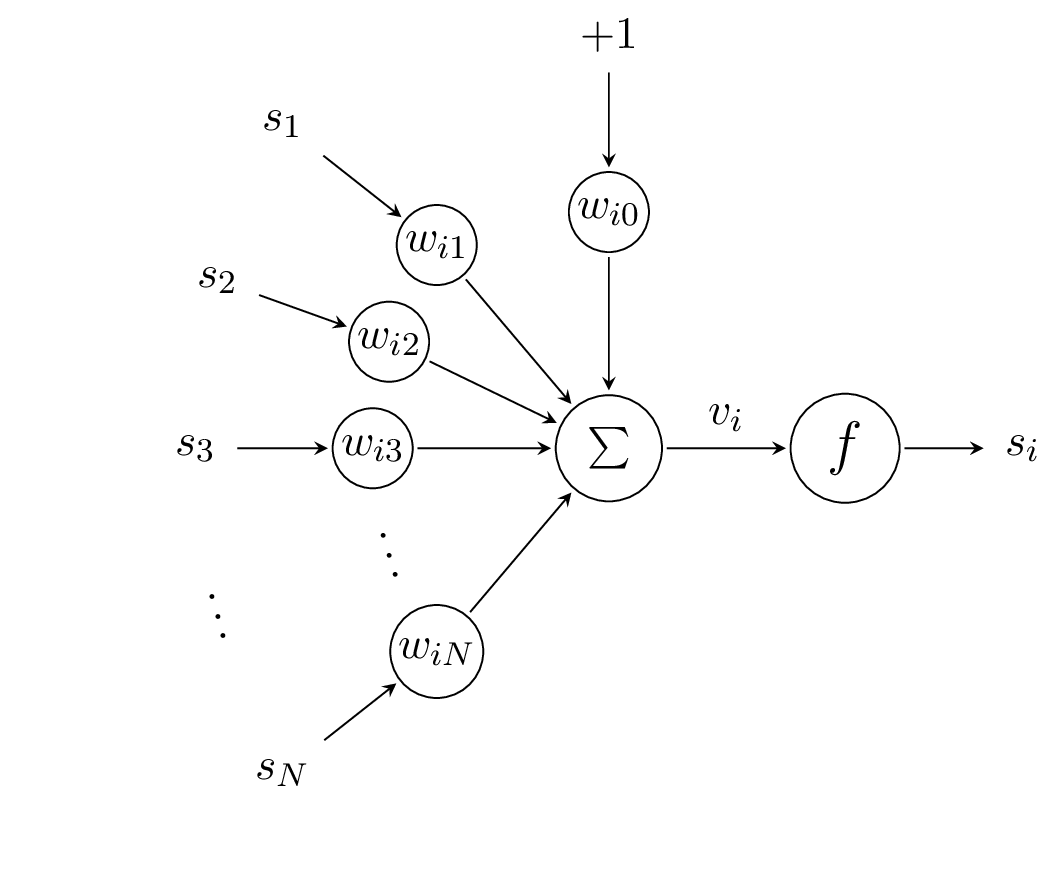
\includegraphics[width=.6\textwidth]{figures/fig_neurona/neurona.pdf}
\shorthandoff{<}
\shorthandoff{>}
\tikzsetnextfilename{figures/neurona/neurona}
\begin{tikzpicture}[   % opciones por defecto
  shorten >=1pt,     % acortar la linea en 1pt al final
  shorten <=1pt,     % acortar la linea en 1pt al principio
  - stealth,         % estilo de flecha al final (manual pgf p~210)
  draw=black!100,    % linea negro 100%
  %font=\relscale{0.9}\sffamily
]
  \tikzstyle{weight}=[draw, circle, inner sep=1pt];
  \tikzstyle{guide}=[draw=red!50];
  %
  %\draw[guide] ([shift={(90:5.5)}]7,0) arc (90:270:5.5);
  % arco que contiene las entradas
  \path ([shift={(150:5.5)}]7,0) arc (150:210:5.5)
  node [pos=0]    (s1) {$s_{1}$}
  node [pos=0.25] (s2) {$s_{2}$}
  node [pos=0.5]  (s3) {$s_{3}$}
  node [sloped, allow upside down, pos=0.75] {$\ldots$}
  node [pos=1]    (sN) {$s_{N}$};
  %% % arco que contiene las entradas
  %% \path ([shift={(135:4)}]5,0) arc (135:225:4)
  %%   node [pos=0]    (s1) {$s_{1}$}
  %%   node [pos=0.25] (s2) {$s_{2}$}
  %%   node [pos=0.5]  (s3) {$s_{3}$}
  %%   node [sloped, allow upside down, pos=0.75] {$\ldots$}
  %%   node [pos=1]    (sN) {$s_{N}$};
  %% %
  %\draw[guide] ([shift={(90:3)}]6,0) arc (90:270:3);
  % arco que contiene los pesos
  \path ([shift={(145:3)}]6,0) arc (145:215:3)
  node [weight,pos=0]    (w1) {$w_{i1}$}
  node [weight,pos=0.25] (w2) {$w_{i2}$}
  node [weight,pos=0.5]  (w3) {$w_{i3}$}
  node [sloped, allow upside down, pos=0.75] {$\ldots$}
  node [weight,pos=1]    (wN) {$w_{iN}$};
  %
  %% % arco que contiene los pesos
  %% \path ([shift={(135:2.2)}]5,0) arc (135:225:2.2)
  %%   node [weight,pos=0]    (w1) {$w_{i1}$}
  %%   node [weight,pos=0.25] (w2) {$w_{i2}$}
  %%   node [weight,pos=0.5]  (w3) {$w_{i3}$}
  %%   node [sloped, allow upside down, pos=0.75] {$\ldots$}
  %%   node [weight,pos=1]    (wN) {$w_{iN}$};
  %% %
  % nodo suma  
  \node [draw, circle, font=\LARGE] (sum) at (5,0) {$\sum$};
  %
  % conexiones entrada - peso y peso - suma
  \foreach \w in {1,2,3,N} {
    \path (s\w) edge (w\w);
    \path  (w\w) edge (sum);
  }
  %
  % peso umbral
  %\draw[guide] ([shift={(180:3)}]5,-1) arc (180:0:3);
  \path ([shift={(90:3)}]5,-1) node [weight] (w0) {$w_{i0}$};
  %% \path ([shift={(90:1.5)}]5,0) node [weight] (w0) {$w_{i0}$};
  \draw[] (w0) -- (sum);
  %
  % entrada +1
  %\draw[guide] ([shift={(180:5.5)}]5,-2) arc (180:0:5.5);
  \path ([shift={(90:5.5)}]5,-2) node [] (plus1) {$+1$};
  \draw[] (plus1) -- (w0);
  %
  % funcion activacion
  %\draw[guide] ([shift={(90:3)}]4,0) arc (90:-90:3);
  \node [draw, circle, font=\large] (fun) at (7,0) {$f$};
  \draw[] (sum) -- (fun) node [pos=0.5, above] {$v_i$};
  %
  % salida s_i
  %\draw[guide] ([shift={(90:5.5)}]3,0) arc (90:-90:5.5);
  \node [] (out) at (8.5,0) {$s_i$};
  \draw[] (fun) -- (out);
  %
  % nodo vacio para separar imagen
  \node at (0,-3.5) {};
\end{tikzpicture}
\shorthandon{<}
\shorthandon{>}


\caption{\captionStyle\protect\label{fig:neurona} El modelo de una neurona.}
\end{figure}
%
%
\subsection{La arquitectura del perceptrón multicapa}
%
El perceptrón multicapa tiene una arquitectura acíclica organizada en
\e{capas}.
La primer capa se denomina \e{capa de entrada} y contiene, en lugar de
neuronas, nodos sensores que ``leen'' el vector presentado como
entrada a la red.
Los valores de las salidas de esta capa equivalen a los componentes
del vector.
Las capas subsiguientes contienen neuronas, cada una de las cuales
recibe como entrada \e{todas} las salidas de la capa anterior.
Para el cálculo de las salidas de cada capa se requiere conocer los
valores de las salidas de la capa anterior, por lo que se dice que el
vector de entrada se \e{propaga hacia adelante} a través de la red.

La salida global de la red se compone por las salidas de las neuronas
en la última capa, denominada simplemente \e{capa de salida}.
Las capas que no son ni de entrada ni de salida se denominan \e{capas
  ocultas}.

En la \iflatexml{}Figura~\ref{fig:mlp}\else\autoref{fig:mlp}\fi{} se
representa un perceptrón multicapa de 2 capas, que lee a su entrada un
vector de 3 elementos.
Este vector es propagado a través de una capa oculta de 4 neuronas
hasta alcanzar las 2 neuronas en la capa de salida, que determinan la
salida de la red.

\begin{figure}[H]
\figureStyle
% 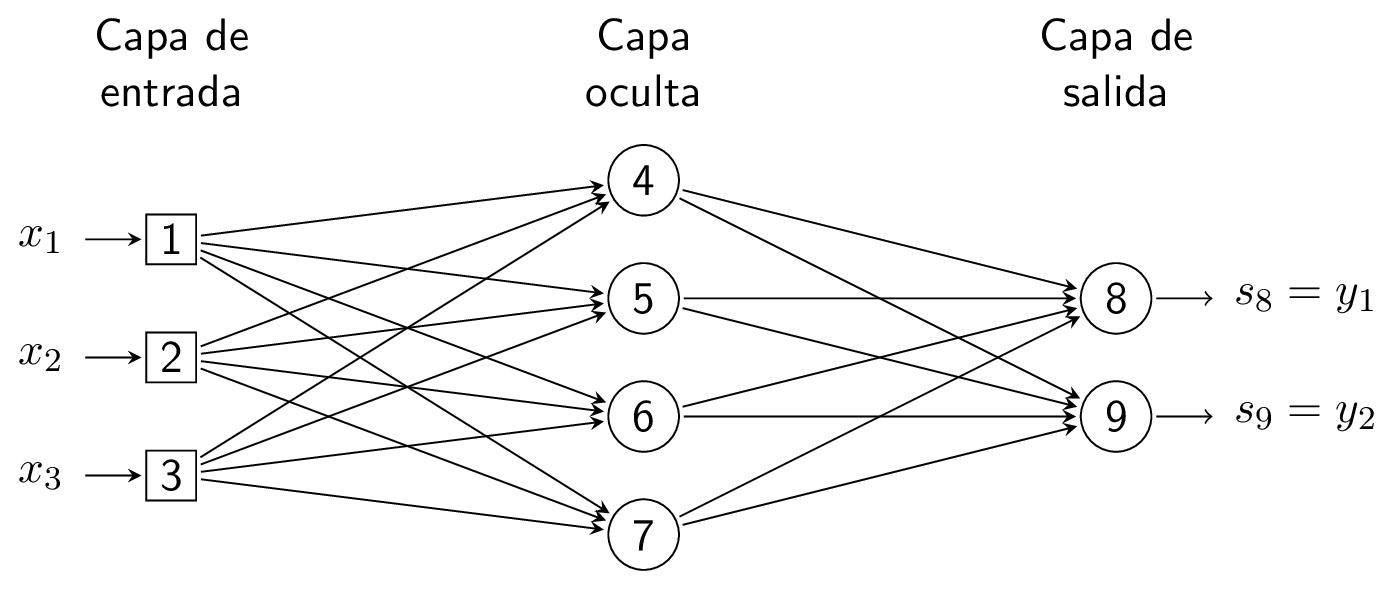
\includegraphics[width=.8\textwidth]{figures/fig_mlp/mlp.pdf}
\def\layersep{4cm}
\def\inputbegin{1}
\def\inputend{3}
\def\hiddenbegin{4}
\def\hiddenend{7}
\def\outputbegin{8}
\def\outputend{9}

\shorthandoff{<}
\shorthandoff{>}
\tikzsetnextfilename{figures/mlp/mlp}
\begin{tikzpicture}[   % opciones por defecto
    shorten >=1pt,     % acortar la linea en 1pt al final
    shorten <=1pt,     % acortar la linea en 1pt al principio
    - stealth,         % estilo de flecha al final (manual pgf p~210)
    draw=black!100,    % linea negro 100%
    node distance=\layersep, % no se que hace esto
    font=\relscale{0.9}\sffamily
  ]

  \tikzstyle{every pin edge}=[stealth -,shorten <=1pt]
  \tikzstyle{neuron}=[draw, minimum size=17pt,inner sep=0pt]
  \tikzstyle{input neuron}=[neuron, minimum size=12pt];
  \tikzstyle{output neuron}=[neuron, circle];
  \tikzstyle{hidden neuron}=[neuron, circle];
  \tikzstyle{annot} = [text width=4em, text centered]

    % Draw the input layer nodes
    \foreach \name / \y in {\inputbegin,...,\inputend}
    % This is the same as writing \foreach \name / \y in {1/1,2/2,3/3,4/4}
        \node[input neuron, pin=left:{$x_\y$}] (N-\name) at (0,-\y) {\y};

    % Draw the hidden layer nodes
    \foreach \name / \y in {\hiddenbegin,...,\hiddenend}
        \path[yshift=\hiddenbegin cm - 0.5cm]
        node[hidden neuron] (N-\name)
        at (\layersep,-\y cm) {\y};

    % Draw the output layer nodes
        \foreach \name[count=\mycount from 1] / \y in {\outputbegin,...,\outputend}
        \path[yshift=\outputbegin cm - 1.5cm]        
        node[output neuron,pin={[pin edge={->}]right:{$s_\y=y_\mycount$}},%
              right of=H-3] (N-\name) at (\layersep,-\y){\y};

    % Connect every node in the input layer with every node in the
    % hidden layer.
    \foreach \source in {\inputbegin,...,\inputend}
        \foreach \dest in {\hiddenbegin,...,\hiddenend}
            \path (N-\source) edge (N-\dest);

    % Connect every node in the hidden layer with the output layer
    \foreach \source in {\hiddenbegin,...,\hiddenend}
        \foreach \dest in {\outputbegin,...,\outputend}
            \path (N-\source) edge (N-\dest);

    % Annotate the layers
    \node[annot,above of=N-\hiddenbegin, node distance=1cm] (hl) {Capa oculta};
    \node[annot,left of=hl] {Capa de entrada};
    \node[annot,right of=hl] {Capa de salida};
    \node[annot] at (0,-4) {};
\end{tikzpicture}
\shorthandon{<}
\shorthandon{>}


\caption{\captionStyle\protect\label{fig:mlp} Perceptrón multicapa.
}
\end{figure}
%
%
\subsection{Entrenamiento}
%
El objetivo del entrenamiento en el perceptrón multicapa es ajustar
los pesos de la red de forma que ésta efectúe la transformación
expresada por el conjunto de entrenamiento $D=(\xx(n),\yy(n))$,
$n=1,\ldots,\ell$.
La diferencia entre las salidas deseadas y las salidas efectivas de la
red se mide con la función de \e{energía} del error $E$:
%
\begin{align}\label{e2:energy-function}
  E = \frac{1}{2}\sum_{j=1}^{\ell}\|\yy_j-\hat{\yy}_j\|,
\end{align}
%
en donde $\hat{\yy}_j$ es el vector formado con las salidas de cada
neurona de la capa de salida.
La función $E$ puede interpretarse como una medida de {aptitud} de los
pesos de la red al conjunto $D$, de modo que satisfacer el objetivo
del aprendizaje es equivalente a encontrar un mínimo global de $E$.
La discusión a continuación se basa en aquella presentada en
\cite[Capítulo~4]{haykin}.

Considerando una neurona $i$ en la capa de salida, sea $s_i(n)$ la
salida de la misma en respuesta al estímulo $\xx(n)$ aplicado en la
capa de entrada.
La \e{señal de error} producida en la salida de esta neurona viene
dada por
%
\begin{align}\label{e2:error-signal-neuron} %4.2
  e_i(n)=y_{k}(n)-s_{i}(n)
\end{align}
%
en donde $y_k(n)$ es la componente del vector de respuesta deseada
$\yy(n)$ correspondiente a la posición de la neurona $i$ en la capa de
salida.
%% en donde $y_{i}$ es el $i$-ésimo elemento del vector de respuesta
%% deseada $\yy$.
La \e{energía de error instantáneo} de la neurona $i$ se define según
%
\begin{align}\label{e2:error-energy-neuron} %4.3
  \C{E}_i(n)=\frac{1}{2}e^2_i(n).
\end{align}
%
Sumando las contribuciones error-energía de todas las neuronas en la
capa de salida, se expresa la \e{energía total de error instantáneo}
de la red como
%
\begin{align}\label{e2:error-energy-net} %4.4
  \C{E}(n)&=\sum_{i\in C}\C{E}_i(n) \\
  &=\frac{1}{2}\sum_{i\in C}e^2_i(n).
\end{align}
%
Aquí, el conjunto $C$ contiene los índices de las neuronas en la capa
de salida.
La energía de error promedio sobre el conjunto de entrenamiento viene
dada por
%
\begin{align}\label{e2:average-energy-net} %4.5
  \C{E}_{\T{av}}&=\frac{1}{\ell}\sum_{n=1}^\ell\C{E}(n) \\
  \tab=\frac{1}{2\ell} \sum_{n=1}^\ell \sum_{i\in C}e^2_i(n).
\end{align}
%
Naturalmente, tanto la energía de error instantáneo como la energía de
error promedio son funciones de todos los pesos sinápticos de la red.
Esta dependencia funcional no fue incluida de forma explícita en la
definición de $\C{E}(n)$ y $\C{E}_{\T{av}}$ en pos de simplificar la
notación.

%
\subsubsection{Aprendizaje en línea y aprendizaje por época}
%
El aprendizaje en línea y el aprendizaje por época hacen referencia
a dos estrategias de entrenamiento que difieren según
el momento en que se efectúa la actualización de los pesos de la
red:
%
\begin{itemize}
\item En el aprendizaje en línea, o aprendizaje por patrón, se efectúa una
  actualización de los pesos de la red inmediatamente
  luego de calcular la salida y el
  error instantáneo de cada ejemplo del conjunto de aprendizaje.
  Esto implica que se efecúan tantas actualizaciones como ejemplos haya
  en el conjunto de entrenamiento.
  Este método funciona especialmente bien
  para grandes conjuntos de entrenamiento que contengan información
  redundante.
\item En el aprendizaje por época (\e{batch learning}),
  la actualización de los pesos de la red
  se efectúa una vez que han sido calculadas las salidas de todos los
  patrones en el conjunto de entrenamiento, minimizando la función de
  error promedio $\C{E}_{\T{av}}$.
\end{itemize}
%
Mientras que el aprendizaje en línea resulta idóneo para situaciones en donde
se requiere una adaptación continua de la máquina de aprendizaje, el
aprendizaje por época redunda en superficies de error más estables, ya que
se promedia todo el conjunto de datos.
En el presente trabajo, se considera en todos los casos el aprendizaje
por época.

%% Los procedimientos adaptativos descritos en adelante
%% utilizan este tipo de aprendizaje, ya que la información de gradiente
%% sumada contiene información más fiable acerca de la forma de la
%% función de error como un todo \cite{riedmiller}.  Algunos autores, sin
%% embargo, sugieren que la mejor técnica es la del aprendizaje en línea
%% \cite{haykin}.

%% %
%% \subsubsection{Técnicas adaptativas}
%% %
%% A la fecha, se han propuesto muchas técnicas para afrontar los
%% problemas inherentes del método de descenso por gradiente. La mayoría
%% tienen sus bases de la disciplina de la teoría de
%% optimización.

%% Estas técnicas se pueden dividir en dos
%% categorías. Aquellos algoritmos que utilizan un conocimiento global
%% del estado de la red como un todo, tal como la dirección del vector de
%% actualización de los pesos ``entero'', son llamadas técnicas globales.
%% Existen muchos ejemplos donde los algoritmos de aprendizaje utilizan el
%% conocimiento global \cite{salomon,moeller}.

%% Por contraste, las estrategias de adaptación locales se basan
%% únicamente en información específica a los pesos, tal como el
%% comportamiento temporal de la derivada parcial de este peso. El
%% enfoque local se relaciona más naturalmente con el concepro de
%% procesamiento distribuido en el que los cálculos pueden efectuarse en
%% paralelo.  Más aún, en muchos casos se encuentra que las estrategias
%% locales funcionan mucho mejor que las globales, a pesar del hecho que
%% utilizan menos información y de que normalmente son mucho más rápidas
%% y fáciles de calcular \cite{schiffmann}.

%
%
\subsection{El algoritmo de retropropagación}
%
El algoritmo de retropropagación es la forma básica de entrenamiento
del perceptrón multicapa, y se basa en ajustar progresivamente los
pesos $w_{ij}$ de la red a partir de la información del gradiente de
la función de error $\nabla\C{E}(n)$.
En cada iteración $n=1,\ldots,\ell$ el algoritmo calcula el error
instantáneo $\C{E}(n)$ de la red sobre el ejemplo $(\xx(n),\yy(n))$, y
aplica una corrección $\Delta{}w_{ij}(n)$ a los pesos sinápticos
$w_{ij}$ proporcional a la derivada parcial
$\dpar{\C{E}(n)}{w_{ij}}{}$.
% Esta forma de entrenamiento se llama \e{entrenamiento en línea}.

Según la regla de la cadena, la derivada $\dpar{\C{E}(n)}{w_{ij}}{}$
puede escribirse
%
\begin{align}\label{e2:deriv-E-wrt-w-expanded}
  \dpar{\C{E}(n)}{w_{ij}}{} = \dpar{\C{E}(n)}{s_i(n)}{}
  \dpar{s_i(n)}{v_i(n)}{} \dpar{v_i(n)}{w_{ij}}{}.
\end{align}
%
Diferenciando ambos lados de (\ref{e2:error-energy-neuron}) respecto
de $s_i(n)$, se tiene
%
\begin{align}\label{e2:deriv-E-wrt-s}
  \dpar{\C{E}(n)}{s_i(n)}{} = -e_i(n).
\end{align}
%
Por (\ref{e2:neuron-general}), se tiene
%
\begin{align}\label{e2:deriv-s-wrt-v}
  \dpar{s_i(n)}{v_i(n)}{} \tab = f'(v_i(n)),\tabs
  \dpar{v_i(n)}{w_{ij}}{} \tab = s_j(n).
\end{align}
%
Reemplazando (\ref{e2:deriv-E-wrt-s})--(\ref{e2:deriv-s-wrt-v}) en
(\ref{e2:deriv-E-wrt-w-expanded}), se tiene
%
\begin{align}\label{e2:deriv-E-wrt-w}
  \dpar{\C{E}(n)}{w_{ij}}{} = -e_i(n) f'(v_i(n)) s_j(n).
\end{align}
%
Cuando la neurona $i$ está en la capa de salida, esta fórmula se
utiliza directamente para el cálculo de $\dpar{\C{E}(n)}{w_{ij}}{}$,
ya que la señal de error $e_i(n)$ de la neurona viene dada por la
diferencia entre el valor deseado $y_k(n)$ y la salida de la neurona
$s_i(n)$ según (\ref{e2:error-energy-neuron}).

Cuando la neurona $i$ se ubica en una capa oculta, el cálculo de
$\dpar{\C{E}(n)}{w_{ij}}{}$ resulta más complejo, ya que no existe una
``respuesta deseada'' correspondiente $y_k(n)$.
Para calcular la derivada $\dpar{\C{E}(n)}{s_{i}}{}$ correspondiente a
una neurona oculta $i$, se supone que el valor de
$\dpar{\C{E}(n)}{s_r}{}$ es conocido para todas las neuronas $r$ de la
capa siguiente a la neurona $i$.
Si $\C{S}(i)$ contiene los índices $r$ de estas neuronas, se puede ver
que
%
\begin{align}
  \dpar{\C{E}}{s_i}{} \tab= \sum_{r\in\C{S}(i)}
      \dpar{\C{E}}{s_r}{}\dpar{s_r}{s_i}{} \notag\\
    \tab= \sum_{r\in\C{S}(i)}
      \dpar{\C{E}}{s_r}{}\dpar{s_r}{v_r}{}\dpar{v_r}{s_i}{} \notag\\
    \tab= \sum_{r\in\C{S}(i)} \dpar{\C{E}}{s_r}{} s'(v_r) w_{ri}.
    \label{e2:deriv-E-wrt-s-hid}
\end{align}
%
Reemplazando (\ref{e2:deriv-E-wrt-s-hid}) y (\ref{e2:deriv-s-wrt-v})
en (\ref{e2:deriv-E-wrt-w-expanded}), se tiene entonces
%
\begin{align}\label{e2:deriv-E-wrt-w-hid}
  \dpar{\C{E}(n)}{w_{ij}}{} =
  \sum_{r\in\C{S}(i)} \dpar{\C{E}(n)}{s_r(n)}{} s'(v_r(n)) w_{ri}
  f'(v_i(n)) s_j(n).
\end{align}
%
Esta fórmula es la clave del algoritmo de retropropagación: por la
arquitectura del perceptrón multicapa, la salida $s_i(n)$ de una
neurona oculta ejerce una influencia en la salida de todas las
neuronas en las capas posteriores.
Similarmente, el \e{gradiente local} de la señal de error de la
neurona viene determinado por los gradientes de error de todas las
neuronas en las capas subsiguientes.

Comenzando el cálculo de $\dpar{\C{E}(n)}{w_{ij}}{}$ por la capa de
salida (\ref{e2:deriv-E-wrt-w}) y continuando con las capas ocultas en
orden inverso (\ref{e2:deriv-E-wrt-w-hid}), el gradiente resulta
calculable para todas las neuronas.
Éste es el origen del nombre ``retropropagación'': se dice que la
información del gradiente de error se propaga hacia atrás, desde la
capa de salida hasta la primer capa oculta.
El desarrollo del algoritmo de retropropagación a mediados de los años
$80$ representó un hito en el campo de las redes neuronales, ya que
brindó un método computacionalmente eficiente para entrenar el
perceptrón multicapa \cite{haykin}.

En pos de simplificar la notación, la descripción del algoritmo de
retropropagación se ha efectuado siguiendo una estrategia de
aprendizaje \e{en línea}, en la que en cada iteración $n$ se presenta
un ejemplo $(\xx(n),\yy(n))$, se calcula la salida de la red
$\hat{\yy}(n)$ y se ajustan los pesos $\ww_{ij}$ según la derivada del
error instantáneo $\C{E}(n)$.
Otra estrategia de entrenamiento posible es el aprendizaje \e{por
  época} (en inglés \e{batch learning}), que consiste en ajustar los
pesos de la red a partir de la derivada de la función de error
promedio $\C{E}_{\T{av}}$.
Para ello, en cada iteración $t$ se obtienen las salidas de la red
para todo el conjunto de entrenamiento $D$, luego se calcula la
función de error promedio, y finalmente se ajustan los pesos
$\ww_{ij}$ de la red en proporción a la derivada
$\dpar{\C{E}_{\T{av}}(t)}{w_{ij}}{}$.

%
\subsubsection{Ajuste de los pesos de la red}
%
En el caso del entrenamiento en línea, en cada paso del entrenamiento
$t$ se calcula la respuesta de la red
$\B{s}(t)$ para la entrada $\xx(t)$ y luego se calcula el gradiente
$\dpar{\C{E}(t)}{w_{ij}}{}$ propagando hacia atrás la señal de error $\C{E}(t)$.
A partir de la información del gradiente
se aplica una corrección $\Delta{}w_{ij}(t)$ sobre el peso
$w_{ij}(t)$, según la ``regla delta''
%
\begin{align}
\label{e2:delta-rule}
  \Delta w_{ij}(t)\tab=-\eta\dpar{\C{E}(t)}{w_{ij}}{},
\end{align}
%
en donde $\eta$ es el parámetro \e{velocidad de aprendizaje} del
algoritmo de retropropagación. La utilización del signo menos en la
\iflatexml{}Ecuación~\ref{e2:deriv-E-wrt-w}
\else\autoref{e2:deriv-E-wrt-w}\fi{} indica el \e{descenso por
  gradiente} en el espacio de los pesos $w_{ij}$. Esto implica que el
ajuste efectuado modifica los pesos en la dirección que reduce el
valor de $\C{E}(t)$.

%
\subsubsection{Entrenamiento por época}
%
En una estrategia de entrenamiento por época, en cada iteración $t$
se propagan hacia adelante todos los vectores $\xx(n)$ del conjunto
de entrenamiento $D$, y a partir de los respectivos
gradientes de error instantáneo $\dpar{\C{E}(n)}{w_{ij}}{}$
se obtiene la energía de error promedio $\C{E}_{\T{av}}$
(\iflatexml{}Ecuación~\ref{e2:average-energy-net}\else\autoref{e2:average-energy-net}\fi)
para la época $t$.

El gradiente de error promedio para la época viene dado por
%
\begin{align}\label{e2:deriv-Eav-wrt-w}
  \dpar{\C{E}_{\T{av}}(t)}{w_{ij}}{}\tab=
  \frac{1}{\ell}\sum_{n=1}^\ell\dpar{\C{E}(n)}{w_{ij}}{},
\end{align}
%
y la corrección a aplicar a los pesos viene dada por
%
\begin{align}\label{e2:delta-rule-epoch}
  \Delta w_{ij}(t)\tab=-\eta\dpar{\C{E}_{\T{av}}(t)}{w_{ij}}{}.
\end{align}
%
Dado que la función $\C{E}_{\T{av}}$ promedia todos los patrones de la
época, la superficie de la función de error resultante es más
``suave'' y el gradiente $\nabla\C{E}_{\T{av}}$ es numéricamente más
estable que en el caso del error intantáneo.

%
\subsubsection{Criterio de corte}
%
En general, no existe un criterio de corte bien definido para
detener el entrenamiento. Algunos criterios razonables para establecer
la convergencia pueden ser:
%
\begin{itemize}
\item Cuando la norma del gradiente es muy pequeña
  ($\|\nabla\C{E}\|\leq\epsilon$), probablemente se deba a que se
  alcanzó un mínimo local de la función de error.
\item Cuando la función de energía promedio $\C{E}_{\T{av}}$ varía muy
  poco entre épocas, también podría significar que se alcanzó un
  mínimo local, indicando convergencia.
\end{itemize}
%
El problema de estos criterios es similar al de la velocidad de
aprendizaje: los valores de tolerancia a considerar para la
convergencia serán siempre dependientes del problema, y una elección
incorrecta puede llevar ya sea a un corte prematuro del entrenamiento,
o bien a que el algoritmo nunca converja.

Un criterio de convergencia alternativo, ampliamente utilizado, se
basa en la aplicación del método de retención sobre el conjunto de
entrenamiento $D$, entrenando sobre un conjunto de estimación $E$ y
evaluando en cada iteración el error sobre un conjunto de validación
$V$ que estima el error de generalización.  El entrenamiento se
detiene cuando se observa que este error es adecuado, o bien cuando
resulta evidente que ha alcanzado su mínimo.

%
\subsection{Variantes del algoritmo de retropropagación}
%
Las técnicas descriptas a continuación son variantes del algoritmo de
retropropagación que intentan sortear algunas de las dificultades
inherentes al descenso por gradiente de la función de error mediante
la utilización de reglas alternativas para la actualización de los
pesos de la red.
En adelante, se utiliza la notación $\C{E}(t)$ para indicar la función
de error, y se observa que para el caso del entrenamiento por época
$\C{E}(t)$ refiere simplemente a $\C{E}_{av}(t)$.

%
\subsubsection{Término de momento}
%
Una estrategia propuesta para incrementar la velocidad de aprendizaje
y mejorar la estabilidad del algoritmo de retropropagación consiste en
modificar la regla delta
(\iflatexml{}Ecuación~\ref{e2:delta-rule}\else\autoref{e2:delta-rule}\fi)
añadiendo un \e{término de momento}
%
\begin{align}\label{e2:momentum-term}
  \Delta w_{ij}(t)\tab=-\eta\dpar{\C{E}(t)}{w_{ij}}{} +\mu\Delta
  w_{ij}(t-1).
\end{align}
%
El término de momento simplemente añade una fracción $\mu$ del paso
anterior $t-1$ al paso actual $t$: si el gradiente mantiene su
orientación, el efecto del término de momento es aumentar la velocidad
de aprendizaje; si en cambio el gradiente cambia de dirección, el
momento ``suaviza'' las oscilaciones.
El \hparam{} de momento $0<\mu<1$ se determina mediante prueba y error
para cada problema.

%
\subsubsection{Descenso más pronunciado}
%
%% En la ``regla delta'' básica
%% (\iflatexml{}Ecuación~\ref{e2:delta-rule}\else\autoref{e2:delta-rule}\fi),
%% la dirección de búsqueda del mínimo
%% viene dada por el negativo del gradiente
%% $-\nabla\C{E}(n)=-\dpar{\C{E}(n)}{w_{ij}}{}$, mientras que la
%% velocidad de aprendizaje $\eta$ determina la magnitud del paso a
%% efectuar.
La regla llamada del \e{descenso más pronunciado} consiste
en buscar, en cada iteración, una velocidad de aprendizaje óptima
$\eta(t)$ mediante una estrategia iterativa denominada \e{búsqueda en
  la línea}.
Básicamente, la búsqueda en la línea consiste en evaluar
la función de error resultante para distintos $\eta$ hasta encontrar
el óptimo.
La regla de actualización de los pesos para esta estrategia es
%
\begin{align}\label{e2:delta-rule-steepest}
  \Delta w_{ij}(t)\tab=-\eta(t)\nabla{\C{E}(t)}.
\end{align}
%
La optimización de $\eta(t)$ añade complejidad computacional a cada
iteración, aunque en general resulta en una reducción del número de
iteraciones necesarias hasta alcanzar la convergencia.
Desde el punto de vista del usuario, evita la necesidad de determinar
el parámetro de entrenamiento $\eta$ mediante prueba y error.

%
\subsubsection{Gradiente conjugado}
%
Al utilizar la regla del descenso más pronunciado, puede demostrarse
que dos pasos de actualización sucesivos ocurren necesariamente en
direcciones perpendiculares.  Esta perpendicularidad entre iteraciones
genera un ``zigzagueo'' en el camino del descenso del gradiente. El
algoritmo del \e{gradiente conjugado} aprovecha esta perpendicularidad
estableciendo como dirección de búsqueda una combinación de la
dirección de búsqueda anterior y del gradiente actual, ``atravesando''
el zigzag y logrando entonces pasos más pronunciados y directos.  La
regla de actualización de los pesos mediante gradiente conjugado viene
dada por
%
\begin{align}\label{e2:delta-rule-conjugate}
  \Delta w_{ij}(t)\tab=\eta(t)\B{d}(t), \tabs
  \B{d}(t)\tab=-\nabla{\C{E}(t)}+\beta\B{d}(t-1),
\end{align}
%
donde $\eta(t)$ se determina mediante búsqueda en la línea y $\beta$
viene dado por la fórmula de Polak-Ribière:
%
\begin{align}\label{e2:polak-ribiere}
  \beta=
  \frac{(\nabla{\C{E}(t)}-\nabla{\C{E}(t-1)})\nabla{\C{E}(t)}}{(\nabla{\C{E}(t-1)})^2}.
\end{align}
%
El mayor costo computacional de las iteraciones en el algoritmo del
gradiente conjugado se compensa con una convergencia mucho más rápida
en problemas de clasificación binarios en comparación con la
retropropagación clásica.

%
\subsubsection{Gradiente conjugado escalado}
%
La estrategia del gradiente conjugado escalado (\e{scaled conjugate
  gradient, SCG}) \cite{scg} es una mejora de la estrategia del
gradiente conjugado estándar que evita la necesidad de optimizar
$\eta(t)$ en cada iteración, ya que determina el paso óptimo a partir
de una aproximación de la segunda derivada de la función $\C{E}$.
Los detalles de la derivación del método pueden encontrarse en
\cite{scg}.
En la actualidad, el algoritmo SCG es una de las estrategias de
entrenamiento más utilizadas debido a su estabilidad y velocidad de
entrenamiento.

%
\subsubsection{Rprop}
%
El algoritmo Rprop \cite{rprop} es una variante heurística sencilla
del algoritmo de retropropagación clásico, que actualiza cada uno de
los pesos de la red de forma independiente.
%% A diferencia de los
%% algoritmos vistos anteriormente, Rprop considera únicamente el signo
%% del gradiente para cada peso, ignorando su magnitud.
Para cada peso $w_{ij}$, Rprop determina un valor de actualización
específico $\Delta{}w_{ij}$ según la siguiente regla basada en el
signo de la derivada parcial
%
\begin{align}
  \Delta{}w_{ij}(t) =
  \begin{cases}
    -\Delta_{ij}^{(t)}, & \T{si}\,\,\,\dpar{\C{E}}{w_{ij}}{}(t) > 0, \\
    +\Delta_{ij}^{(t)}, & \T{si}\,\,\,\dpar{\C{E}}{w_{ij}}{}(t) < 0, \\
    0, & \T{en otro caso}.
  \end{cases}
\end{align}
%
El algoritmo regula su funcionamiento mediante dos hiperparámetros,
$\Delta_0$ y $\Delta_{\max}$, que especifican respectivamente el valor
de inicialización de todos los $\Delta_{ij}$ y la magnitud máxima
permitida para cada $\Delta_{ij}$.
Los valores de cada $\Delta_{ij}$ se modifican en cada iteración según
la regla
%
\begin{align}
  \Delta{}_{ij}^{(t)} \tab =
  \begin{cases}
    \eta^+\,\Delta_{ij}^{(t-1)}, & \T{si}\,\,\,\dpar{\C{E}}{w_{ij}}{} {(t-1)}
      \dpar{\C{E}}{w_{ij}}{} {(t)} > 0, \\
    \eta^-\,\Delta_{ij}^{(t-1)}, & \T{si}\,\,\,\dpar{\C{E}}{w_{ij}}{} {(t-1)}
      \dpar{\C{E}}{w_{ij}}{} {(t)} < 0, \\
    \Delta_{ij}^{(t-1)}, & \T{en otro caso}.
  \end{cases}
  \tabs
  \begin{split}
    \eta^-=0.5, \\
    \eta^+=1.2.
  \end{split}
\end{align}
%
El algoritmo Rprop es una de las técnicas más rápidas y más populares
para el entrenamiento del perceptrón multicapa.
Dada su estabilidad, la elección de los hiperparámetros $\Delta_{0}$ y
$\Delta_{\max}$ no es crítica, y en la práctica se utilizan los
valores preestablecidos $\Delta_{0}=0.1$ y $\Delta_{\max}=50$.

%
%
%
\section{Máquina de vectores de soporte}
%
La máquina de vectores de soporte (\eng{Support Vector Machine, SVM})
es una máquina de aprendizaje propuesta por Boser et al. \cite{boser}
y Cortes y Vapnik \cite{svm} que puede ser utilizada para tareas de
clasificación y regresión. Su funcionamiento se basa en la
construcción de un modelo en el cual los ejemplos son representados
como puntos en el espacio.
En un problema de clasificación, el entrenamiento de la SVM construye,
a partir de los ejemplos en el conjunto de entrenamiento, una frontera
de decisión que permite determinar la pertenencia de clase de los
ejemplos según se ubiquen a un lado u otro de la frontera.

La popularidad de la máquinas de vectores de soporte se debe en gran
parte a que permiten incorporar no-linealidad a la representación
vectorial de los ejemplos de manera eficiente, mediante la utilización
de familias especiales de funciones denominadas núcleos.

%% En su variante más común, la máquina de vectores de soporte incorpora
%% un término de regularización que permite su aplicación a conjuntos de
%% datos no separables y reducir la complejidad de la solución, evitando
%% el sobreajuste.

La máquina de vectores de soporte es un tipo de \e{clasificador
  lineal} con tres propiedades importantes:
%
\begin{enumerate}
\item El algoritmo de entrenamiento de la SVM genera una frontera de
  decisión óptima desde el punto de vista geométrico.
\item Permite efectuar cálculos entre los vectores (ejemplos) de
  manera eficiente mediante la utilización de funciones especiales
  denominadas \e{núcleos}.
\item Permite incorporar regularización al modelo, que evita el
  sobreajuste y al mismo tiempo permite aplicar el clasificador a
  datos no separables.
\end{enumerate}
%
A continuación se presenta una descripción de la SVM
comenzando por el clasificador lineal e incorporando estas propiedades
hasta alcanzar la formulación más general, que
utiliza funciones núcleo e incorpora regularización al modelo.
En esta descripción se trata la obtención del modelo de un
clasificador binario a partir de un conjunto de entrenamiento
$D=\left((\xx_1,y_1),\ldots,(\xx_\ell,y_\ell)\right)$, en donde el
indicador de clase del $i$-ésimo ejemplo toma alguno de los dos
valores posibles $y_i=+1$ o $y_i=-1$.

%
%
\subsection{El clasificador lineal}
%
El clasificador lineal es una máquina de aprendizaje \cite{nilsson}
que sirve como fundamento de la máquina de vectores de soporte. De
hecho, la SVM es en sí misma un tipo particular de
clasificador lineal.

En primer lugar, sea $\BPhi:X\rightarrow{}Z$ una función que
transforma el denominado \e{espacio de entrada} $X$ a otro espacio
vectorial inducido $Z$, denominado \e{espacio imagen}.
A partir del
conocimiento previo del problema, se pretende que la transformación
$\BPhi$ sea tal que los \e{vectores imagen} $\zz=\BPhi(\xx)$ se
ubiquen, según su clase $\yy$, en regiones del espacio $Z$ bien
diferenciadas entre sí.

Entonces, dado un patrón de entrada $\xx\in{}X$, el clasificador
lineal calcula primero el vector imagen $\zz=\BPhi(\xx)$, para luego
asignarle una clase de salida $\hat{y}=\pm{}1$ según sea el signo de
la función discriminante lineal $f=\ww^T\zz+b$. Los valores de $\ww$
y $b$ se determinan en el entrenamiento del clasificador, cuyos detalles
se omiten de la presente descripción.

Por último, se observa que la ecuación $\ww^T\zz+b=0$ define un
hiperplano en el espacio inducido $Z$. Dicho hiperplano determina una
frontera de decisión entre las clases $\hat{\yy}=+1$ e
$\hat{\yy}=-1$. Para visualizarlo, obsérvese que, desde el punto de
vista geométrico, el signo de $\ww^T\zz+b$ determina de qué lado del
plano se encuentra el punto $\zz$.
%
\begin{quote}
  {\bfseries Notación.}\quad{}En la literatura, resulta común
  encontrar que el vector $\zz$ se denomina \e{vector de
    características} (\e{feature vector}) y el espacio vectorial $Z$
  como \e{espacio de las características} (\e{feature space}).  En
  este trabajo se prefiere denominarlos con los nombres alternativos
  \e{vector imagen} y \e{espacio vectorial imagen} para evitar
  confusión con el proceso previo de extracción de características.
\end{quote}
%

%
\subsubsection{Espacio imagen}
%
La primera adición de la SVM al clasificador lineal básico es una
transformación de los vectores de entrada a un \e{espacio imagen}.
Esto se logra aplicando una función $\BPhi:X\rightarrow{}Z$, que
transforma el \e{espacio de entrada} $X$ a otro espacio vectorial
inducido $Z$, llamado \e{espacio imagen}.
La elección de la función $\BPhi$ es tal que los datos transformados
sean separables en el espacio $Z$.
Dada una entrada $\xx\in{}X$, la máquina de vectores de soporte
calcula un vector imagen $\BPhi(\xx)$ y le asigna una clase de
salida $\hat{y}=\pm{}1$ según
%
\begin{align*}
  y = \T{signo}(\ww^T \BPhi(\xx)+b)
\end{align*}
%
Los valores de $\ww$ y $b$ se obtienen del algoritmo de entrenamiento,
que se explicará más adelante.
En este caso, la frontera de decisión se ubica en el espacio imagen
$Z$, y viene dada por el hiperplano con ecuación
$\ww^T\BPhi(\xx)+b=0$.
%
\begin{quote}
  {\bfseries Notación.}\quad{}En la literatura, resulta común
  encontrar que el vector $\BPhi(\xx)$ se denomina \e{vector de
    características} (\e{feature vector}) y el espacio vectorial $Z$
  como \e{espacio de las características} (\e{feature space}).  En
  este trabajo se prefiere denominarlos con los nombres alternativos
  \e{vector imagen} y \e{espacio vectorial imagen} para evitar
  confusión con el proceso previo de extracción de características.
\end{quote}
%

%
%
\subsection{El hiperplano de separación óptimo}
%
Dado un conjunto de entrenamiento
$D=\left((\xx_1,y_1),\ldots,(\xx_\ell,y_\ell)\right)$, se dice que
éste es linealmente separable en el espacio imagen $Z$ cuando existe
una función discriminante lineal $f(\xx)=\ww^T\BPhi(\xx)+b$ tal que su
signo permite determinar sin errores la clase de todos los elementos
del conjunto. Cuando el conjunto $D$ es linealmente separable en $Z$,
se sabe que existen infinitas funciones discriminantes lineales
capaces de clasificar correctamente todos los elementos.

La característica saliente de la máquina de vectores de soporte es
que, durante el entrenamiento, determina un hiperplano de separación
$\ww^T\zz+b=0$ \e{óptimo}, que maximiza la distancia a los puntos
$\zz_i=\BPhi(\xx_i)$ más cercanos. Esto se expresa a través del
problema de optimización
%
\begin{equation}\label{e2:svm-problem-basic}
  \begin{aligned}
    \min_{\ww,b} \quad\tabs \frac{1}{2}\|\ww\|^2, \\
    \T{sujeto a}\quad\tabs y_i f_i\geq1,\,i=1,\ldots,\ell\,.
  \end{aligned}
\end{equation}
%
Aquí, $f_i=f(\xx_i)=\ww^T\BPhi(\xx_i)+b$ es la función discriminante
lineal aplicada al vector $\xx_i$. En términos coloquiales, este
problema puede leerse
%
\begin{align*}
  \min \frac{1}{2}\|\ww\|^2 \quad \tabs \T{encontrar el $\ww$ más
    pequeño según la norma euclídea $\|\cdot\|$}\ldots\\
  |f_i|\geq1 \quad \tabs \T{estableciendo en $1$ la distancia del
    hiperplano a los puntos más cercanos},\\
  y_i\hat{y}_i>0\quad \tabs \T{y tal que la clase $y_i$ coincida con el
    signo del discriminante ($\hat{y}_i=\T{signo}(f_i)$)}.
\end{align*}
%
La distancia de un vector $\zz_i=\BPhi(\xx_i)$ al hiperplano
$\ww^T\zz+b=0$ viene dada por
%
\begin{align*}
  d_i=\frac{\ww}{\|w\|}\cdot\zz_i+b,
\end{align*}
%
por
ello, minimizar $\|w\|$ equivale a maximizar la distancia $d_i$.

Puede demostrarse que el vector solución $\ww_*$ al
Problema~\ref{e2:svm-problem-basic} es una combinación lineal de
aquellos vectores $\zz_i$ para los cuales se cumpla la condición:
%
\begin{align*}
  |\ww^T\zz_i+b\,|=1.
\end{align*}
%
Estos vectores se denominan \e{vectores de soporte}, lo que da el
nombre al clasificador.
Los hiperplanos $\ww^T\zz+b=\pm1$ que contienen los vectores
de soporte conforman el llamado \e{margen} del clasificador.

El Problema~\ref{e2:svm-problem-basic} también puede entenderse como
la maximización de la distancia del hiperplano $\ww^T\zz+b=0$ al
margen $\ww^T\zz+b=\pm1$.
Esto explica el nombre alternativo por el cual se conoce a la máquina
de vectores de soporte: \e{clasificador de margen máximo}.

%% Desde el punto de vista numérico, el problema
%% (\ref{e2:svm-problem-basic}) es un problema de optimización cuadrático
%% convexo con restricciones lineales.

%
%
\subsection{Formulación dual}
%
En el problema (\ref{e2:svm-problem-basic}) se minimiza una función
cuadrática simple con restricciones relativamente complejas
${y}_i(\ww^T\BPhi(\xx_i)+b)\geq{}1$. Utilizando la técnica de los
multiplicadores de Lagrange \cite{bottou,kuhntucker}, resulta posible
obtener una fomulación alternativa del problema con restricciones
simples, cuya conveniencia será aparente con la introducción del
concepto de núcleos.

La técnica de los multiplicadores de Lagrange permite incorporar las
restricciones del problema dentro de la función a optimizar.  En
primer lugar, se define el funcional lagrangiano
%
\begin{align}\label{e2:lagrangian}
  \C{L}(\ww,b,\Balpha) = \frac{1}{2} \|\ww\|^2 + \sum_{i=1}^{\ell}
  \alpha_i (1-y_i(\langle\ww,\BPhi(\xx)\rangle+b)).
\end{align}
%
Como se puede ver, el funcional $\C{L}$ es la función a optimizar más
las restricciones ${y}_if_i\geq{}1$, expresadas en la forma $g(\xx)\leq0$,
y multiplicadas por las variables de holgura $\alpha_i$,
denominadas \e{multiplicadores de Lagrange}. A partir del lagrangiano
se plantea la formulación \emph{dual} del problema
%
\begin{align}\label{e2:svm-problem-dual}
  \begin{split}
    \max_\alpha \tabs\quad f(\Balpha) = \min_{\ww,b} \C{L}(\ww,b,\Balpha)\\
    \T{sujeto a} \tabs\quad \alpha_i \geq 0\T{ para todo } i\in\{1,\ldots,\ell\}.
  \end{split}
\end{align}
%
En este problema las restricciones son más sencillas y
aplican únicamente a los multiplicadores de Lagrange.
Dado que $\frac{1}{2}\|\ww\|^2$ es una función continuamente derivable
y convexa, y dado que $\C{L}$ es continuamente derivable respecto de
sus argumentos en las cercanías del punto óptimo
$(\ww^*,b^*,\Balpha^*)$, las condiciones de Karush-Kuhn-Tucker
\cite{kuhntucker} garantizan la existencia de una solución
$(\ww^*,b^*,\Balpha^*)$ al problema dual
(\iflatexml{}Ecuación~\ref{e2:svm-problem-dual}\else\autoref{e2:svm-problem-dual}\fi)
tal que $(\ww^*,b^*)$ también es solución al problema primal
(\iflatexml{}Ecuación~\ref{e2:svm-problem-basic}\else\autoref{e2:svm-problem-basic}\fi).

Dado que la solución $(\ww^*,b^*,\Balpha^*)$ del problema dual
(\ref{e2:svm-problem-dual}) es un punto de ``silla'', sus respectivas
derivadas parciales se anulan. Esto implica que
%
\begin{align}\label{e2:lagrangian-w}
  \evalen{\ww=\ww^*}{\dpar{\C{L}(\ww,b,\Balpha)}{\ww}{}}
    &=\ww^*-\sum_{i=1}^\ell y_i\alpha_i\BPhi(\xx_i) = 0
    &\Rightarrow \ww^* = \sum_{i=1}^\ell y_i\alpha_i\BPhi(\xx_i),
  \\
  \label{e2:lagrangian-sum-yalpha}
  \evalen{b=b^*}{\dpar{\C{L}(\ww,b,\Balpha)}{b}{}}
    &=-\sum_{i=1}^\ell y_i\alpha_i = 0
      &\Rightarrow \sum_{i=1}^\ell y_i\alpha_i = \yy^T\Balpha = 0.
\end{align}
%
Incorporando los resultados (\ref{e2:lagrangian-w}) y
(\ref{e2:lagrangian-sum-yalpha}) en la
\iflatexml{}Ecuación~\ref{e2:lagrangian}\else\autoref{e2:lagrangian}\fi,
el lagrangiano puede escribirse
%
\begin{align*}
  \C{L}(\ww,b,\Balpha)
  & =
    \frac{1}{2}\sum_{i=1}^\ell\sum_{j=1}^\ell y_iy_j\alpha_i\alpha_j
    \langle\BPhi(\xx_i),\BPhi(\xx_j)\rangle \\
    &\qquad\qquad +
    \sum_{i=1}^{\ell} \alpha_i \left(1-y_i\left(\left\langle
    \sum_{j=1}^\ell y_j\alpha_j\BPhi(\xx_j) ,\BPhi(\xx_i)\right\rangle
    +b\right)\right)\\
  & =
    -\frac{1}{2}\sum_{i=1}^\ell\sum_{j=1}^\ell y_iy_j\alpha_i\alpha_j
    \langle\BPhi(\xx_i),\BPhi(\xx_j)\rangle +
    \sum_{i=1}^{\ell} \alpha_i  - b \sum_{i=1}^\ell y_i\alpha_i \\
 & =
    -\frac{1}{2}\sum_{i=1}^\ell\sum_{j=1}^\ell y_iy_j\alpha_i\alpha_j
    \langle\BPhi(\xx_i),\BPhi(\xx_j)\rangle +
    \sum_{i=1}^{\ell} \alpha_i  .
\end{align*}
%
Con este resultado, se reescribe el problema dual en función de los
multiplicadores de Lagrange $\alpha_i$:
%
\begin{align}
  \begin{split}
    \max_\alpha &\quad
    -\frac{1}{2}\sum_{i=1}^\ell\sum_{j=1}^\ell y_iy_j\alpha_i\alpha_j
    \langle \BPhi(\xx_i),\BPhi(\xx_j) \rangle +
    \sum_{i=1}^{\ell} \alpha_i \\
    \T{sujeto a} &\quad \yy^T\Balpha = 0, \\
    &\quad \alpha_i \geq 0\T{ para todo } i\in\{1,\ldots,\ell\}.
  \end{split}
  \label{e2:svm-problem-dual2}
\end{align}
%
Este problema se resuelve directamente para las variables de holgura
$\alpha_i$, resultando en una solución
$\Balpha^*$. El vector solución $\ww^*$ al problema original
(\ref{e2:svm-problem-basic}) se obtiene por la
 \iflatexml{}Ecuación~\ref{e2:lagrangian-w}\else\autoref{e2:lagrangian-w}\fi:
%
\begin{align}\label{e2:w-from-alpha}
  \ww^* = \sum_{i=1}^\ell y_i\alpha^*_i\BPhi(\xx_i).
\end{align}
%
El cálculo de $b^*$ óptimo se deriva de las condiciones de
complementariedad de Karush-Kuhn-Tucker \cite{kuhntucker,bottou}, que
establecen que para todo $i\in\{1,\ldots,\ell\}$, se cumple
$\alpha^*_i(1-y_i(\langle\ww^*,\BPhi(\xx_i)\rangle+b^*))=0$. Entonces,
para algún $\alpha^*_i\neq0$, se tiene
%
\begin{align}\label{e2:b-from-alpha}
  b^* = y_i - \langle\ww^*,\BPhi(\xx_i)\rangle .
\end{align}
%
La existencia de $\alpha^*_i\neq0$ está garantizada siempre que el
conjunto de entrenamiento tenga elementos de ambas clases
\cite{glasmachers}.

%
%
\subsection{Núcleos}
%
Un núcleo, denominado también por su nombre en inglés \eng{kernel}, es
una función $k:X\times{}X\rightarrow{}\RR$ que generaliza el concepto
de métrica \cite{stewart}.
Dado un par de vectores $\xx_1,\xx_2\in{}X$, un núcleo permite
comparar la similaridad entre los vectores $\BPhi(\xx_1),\BPhi(\xx_2)$
\e{transformados} a un espacio vectorial inducido $Z$, sin necesidad
de calcular la transformación $\BPhi$ de forma explícita.
%
\begin{definicion}[Núcleo]
  Una función $k:X\times{}X\rightarrow{}\R{R}$ se dice un núcleo
  en el conjunto $X$ si cumple con las siguientes propiedades:
  %
  \begin{enumerate}
  \item $k(\xx_1,\xx_2)=k(\xx_2,\xx_1)$ para todo $\xx_1,\xx_2\in{}X$.
  \item Para cada $n\in\R{N}$ y para todos los puntos
    $(\xx_1,\ldots,\xx_\ell)\in{}X^\ell$, la matriz de Gram
    $K\in\R{R}^{\ell\times\ell}$ definida como
    $K_{ij}=k(\xx_i,\xx_j),\,i,j\in\{1,\ldots,\ell\}$ es semidefinida
    positiva.
  \end{enumerate}
  %
\end{definicion}
%
Para un núcleo $k$, el teorema de Mercer \cite{mercer} asegura la
existencia de un espacio de Hilbert $Z$ y una transformación
$\BPhi:X\rightarrow{}Z$ tal que, para cualquier par de vectores
$\xx_i,\xx_j\in{}X$, el núcleo calcula el producto interno de los
mismos en el espacio imagen:
$k(\xx_i,\xx_j)=\langle\BPhi(\xx_i),\BPhi(\xx_j)\rangle$.
%% Es importante tener en cuenta que ni el espacio $F$ ni la
%% transformación $\BPhi$ son únicos.

El teorema de Mercer puede aplicarse directamente a la función
objetivo del problema dual de la SVM (\ref{e2:svm-problem-dual2}),
reemplazando los productos internos
$\left\langle\BPhi(\xx_i),\BPhi(\xx_j)\right\rangle$, por la función
núcleo $k(\xx_i,\xx_j)$.
Esto se llama comúnmente como el ``truco del núcleo'', del inglés
\e{kernel trick}, y da como resultado el problema
%
\begin{align}
  \begin{split}
    \max_\alpha &\quad
    -\frac{1}{2}\sum_{i=1}^\ell\sum_{j=1}^\ell y_iy_j\alpha_i\alpha_j
    k(\xx_i,\xx_j) + \sum_{i=1}^{\ell} \alpha_i \\
    \T{sujeto a} &\quad \yy^T\Balpha = 0, \\
    &\quad \alpha_i \geq 0\T{ para todo } i\in\{1,\ldots,\ell\}.
  \end{split}
  \label{e2:svm-problem-kernel}
\end{align}
%
En este problema, las operaciones de producto interno en el espacio
imagen $Z$ se efectúan a través de la función núcleo $k$, sin
necesidad de calcular la transformación $\BPhi$ en forma explícita.

Desde un punto de vista puramente matemático, la utilización del truco
del núcleo no aporta ninguna ventaja, ya que los algoritmos son
equivalentes.
Desde un punto de vista computacional, sin embargo, la
diferencia es decisiva: utilizando el truco del núcleo, se pueden
calcular productos internos en espacios vectoriales de alta
dimensionalidad --incluso infinita--, sin necesidad de efectuar la
transformación $\BPhi$, cuyo cálculo directo muchas veces resulta
prohibitivo o incluso imposible en un ordenador.

%% Es intuitivamente claro que la elección de un núcleo que represente
%% una métrica específica al problema puede mejorar el rendimiento de las
%% máquinas de aprendizaje. Por ejemplo, en una tarea de clasificación es
%% conveniente elegir una métrica que agrupa las diferentes clases.

A continuación, se presentan algunos núcleos más
utilizados con las máquinas de vectores de soporte.
%
\begin{description}
%
\item[Núcleo lineal]
  %
  \begin{align}
    k(\xx_1,\xx_2)=\langle \xx_1, \xx_2\rangle=\xx_1^T\xx_2
  \end{align}
  %
  Calcula simplemente el producto interno entre sus argumentos.
  Aquí, el espacio imagen $Z$ es el mismo que el espacio de entrada,
  $X$, correspondiente a la transformación identidad $\BPhi(\xx)=\xx$.
%
\item[Núcleo polinómico]
  %
  \begin{align}
    k(\xx_1,\xx_2)=\left(\langle{}\xx_1,\xx_2\rangle+\theta\right)^d,
  \end{align}
  %
  con grado $d\in\R{N}$ y desvío $\theta\in\RR$.
  Este núcleo es una generalización del núcleo lineal (el caso $d=1$ y
  $\theta=0$).
  Su espacio imagen es el espacio de los polinomios de grado $d$ sobre
  el espacio $X$.
  El cálculo del producto interno aplicando el núcleo requiere
  $\C{O}(\dim{}X)$ operaciones, contrastando con las
  $\C{O}\left((\dim{}X)^d\right)$ necesarias para el cálculo de la
  transformación $\BPhi$.
%
\item[Función de base radial (RBF)]
  %
  \begin{align}
    k(\xx_1,\xx_2)=\exp\left(-\frac{\|\xx_1-\xx_2\|^2}{2\sigma^2}\right)
    =\exp\left(-\gamma\|\xx_1-\xx_2\|^2\right)
  \end{align}
  %
  También llamado núcleo gaussiano, o \eng{Radial Basis Function} en
  inglés, es el núcleo más utilizado.
  En la primer forma, el hiperparámetro $\sigma$ se llama parámetro de
  amplitud.
  En la segunda forma el hiperparámetro $\gamma$ se llama de
  concentración.
  La transformación $\BPhi$ correspondiente a este núcleo genera un
  espacio imagen de dimensión infinita, imposible de calcular
  directamente.
  El producto interno mediante este núcleo se puede calcular en
  $\C{O}(\dim{}X)$ operaciones.
  %
\end{description}
%

%
\subsubsection{Funciones núcleo comunes}
%
A continuación, se presentan algunas de las funciones núcleo más
utilizadas con las máquinas de vectores de soporte.
%
\begin{description}[font=\relscale{0.9}]
%
\item[Núcleo lineal]
  %
  \begin{align}
    k(\xx_1,\xx_2)=\langle \xx_1, \xx_2\rangle=\xx_1^T\xx_2
  \end{align}
  %
  Calcula simplemente el producto interno entre sus argumentos.
  Aquí, el espacio imagen $Z$ es el mismo que el espacio de entrada,
  $X$, correspondiente a la transformación identidad $\BPhi(\xx)=\xx$.
%
\item[Núcleo polinómico]
  %
  \begin{align}
    k(\xx_1,\xx_2)=\left(\langle{}\xx_1,\xx_2\rangle+\theta\right)^d,
  \end{align}
  %
  con grado $d\in\R{N}$ y desvío $\theta\in\RR$.
  Este núcleo es una generalización del núcleo lineal (el caso $d=1$ y
  $\theta=0$).
  Su espacio imagen es el espacio de los polinomios de grado $d$ sobre
  el espacio $X$.
  El cálculo del producto interno aplicando el núcleo requiere
  $\C{O}(\dim{}X)$ operaciones, contrastando con las
  $\C{O}\left((\dim{}X)^d\right)$ necesarias para el cálculo de la
  transformación $\BPhi$.
%
\item[Función de base radial (RBF)]
  %
  \begin{align}
    k(\xx_1,\xx_2)=\exp\left(-\frac{\|\xx_1-\xx_2\|^2}{2\sigma^2}\right)
    =\exp\left(-\gamma\|\xx_1-\xx_2\|^2\right)
  \end{align}
  %
  También llamado núcleo gaussiano, o \eng{Radial Basis Function} en
  inglés, es el núcleo más utilizado.
  En la primer forma, el hiperparámetro $\sigma$ se llama parámetro de
  amplitud.
  En la segunda forma el hiperparámetro $\gamma$ se llama de
  concentración.
  La transformación $\BPhi$ correspondiente a este núcleo genera un
  espacio imagen de dimensión infinita, imposible de calcular
  directamente.
  El producto interno mediante este núcleo se puede calcular en
  $\C{O}(\dim{}X)$ operaciones.
  %
\end{description}
%

%
%
\subsection{SVM de margen duro}
%
La máquina de vectores de soporte más simple es aquella llamada ``de
margen duro'', y consiste en un clasificador de margen máximo que
incorpora el ``truco del núcleo''.
Dado un núcleo $k:X\times{}X\rightarrow\RR$,
se asume que el conjunto de datos transformado
$\left((\BPhi(\xx_1),y_1)),\ldots,(\BPhi(\xx_\ell),y_\ell)\right)$ es
linealmente separable en el espacio inducido $Z$.
El entrenamiento consiste en resolver el
problema de optimización (\ref{e2:svm-problem-kernel}), que en
notación vectorial se escribe
%
\begin{align}
  \label{e2:svm-hard-margin}
  \begin{split}
    \max_{\Balpha}\quad\tabs
      \B{1}^T\Balpha-\frac{1}{2}\Balpha^T\QQ\Balpha\\
    \T{sujeto a} \quad\tabs
      \yy^T\Balpha = 0, \\
      \tabs \alpha_i\geq 0,  i\in {1,\ldots,\ell }.
  \end{split}
\end{align}
%
La matriz $\QQ$ es semidefinida positiva con elementos por
$Q_{ij}=y_iy_jk(\xx_i,\xx_j)$, y $\B{1}$ es un vector columna de
$\ell$ elementos iguales a $1$.  El entrenamiento de este problema se
efectúa comúnmente mediante el algoritmo denominado SMO
(\eng{Sequential Minimal Optimization}, Optimización Mínima
Secuencial) \cite{smo} específicamente diseñado para la SVM, aunque
puede ser resuelto mediante cualquier algoritmo capaz de resolver un
problema de optimización cuadrático.

El modelo de la máquina de vectores de soporte de margen
duro viene dado por
%
\begin{align}
  \begin{split}
    h(\xx) &= \T{signo}\left(\langle\ww^*,\BPhi(\xx)\rangle+b^*\right).
  \end{split}
\label{e2:svm-model-hard0}
\end{align}
%
Para el cálculo de $h(\xx)$, se utiliza la función núcleo $k$ y se
observa que
%
\begin{align}
  \langle\ww^*,\BPhi(\xx)\rangle \tab=
  \sum_{i=1}^\ell{}y_i\alpha^*_ik(\xx_i,\xx),\\
  b^* \tab= y_j - \sum_{i=1}^\ell{}y_i\alpha^*_ik(\xx_i,\xx_j).
  \label{e2:svm-model-b-kernel}
\end{align}
%
El subíndice $j$ de la
\iflatexml{}Ecuación~\ref{e2:svm-model-b-kernel}\else\autoref{e2:svm-model-b-kernel}\fi{}
es cualquiera que cumpla con la condición $\alpha_j>0$.  Con estos
resultados, el modelo $h(\xx)$ se escribe
%
\begin{align}
  h(\xx) &=
  \T{signo}\left(\sum_{i=1}^\ell{}y_i\alpha^*_ik(\xx_i,\xx)+b^*\right).
\label{e2:svm-model-hard}
\end{align}
%

%
%
\subsection{SVM de margen blando}
%
La máquina de vectores de soporte llamada ``de margen blando''
incorpora regularización al modelo, permitiendo la clasificación
errónea de algunos ejemplos de entrenamiento.
%% Al aplicar regularización, los modelos resultantes son más simples, y
%% además, permite entrenar el clasificador con datos de entrenamiento
%% que no son separables.
%
%% En la máquina de vectores de soporte sin regularización (``margen
%% duro''), el objetivo del entrenamiento es reducir la complejidad del
%% modelo resultante: esto puede verse a partir de la interpretación
%% geométrica de $\ww$: una gran norma de $w$ corresponde a un pequeño
%% margen geométrico $\rho=1/\|\ww\|$, y consecuentemente a un modelo más
%% complejo.
Esto se logra agregando al objetivo de minimización una medida del
error de clasificación de cada ejemplo $(\xx_i,y_i)$ a través de una
variable de holgura no negativa $\xi_i$, que es la función de pérdida
``bisagra''
%
\begin{align}
  \xi_n = \max\{0,1-y_n(\langle{}\ww,\Phi(\xx_i)\rangle+b)\}.
\end{align}
%
La variable $\xi_i$ mide la violación funcional del margen para cada
ejemplo $(\xx_i,y_i)$, indicada por la distancia al hiperplano de
separación. Por definición, $\xi_i$ es mayor a cero sólo cuando el
modelo clasifica incorrectamente el ejemplo, esto es, cuando
$h(\xx_i)\neq{}y_i$.

Se introduce un hiperparámetro de regularización $C>0$ que ajusta el
balance entre complejidad del modelo y la cantidad de error, lo que deriva
en el problema de optimización \emph{primal}
%
\begin{align}
  \label{svm-primal-blando}
  \begin{split}
    \min_{(\ww,b,\xi)} \quad & \frac{1}{2}\|\ww\|^2+C\sum_{i=1}^{\ell}\xi_i\\
    \T{sujeto a} \quad &
    y_i\left(\langle{}\ww,\BPhi(\xx_i)\rangle+b\right) \geq 1-\xi_i, i=1,\ldots,\ell, \\
    & \xi_i \geq 0, i=1,\ldots,\ell.
  \end{split}
\end{align}
%

%% La SVM de margen blando (con regularización ``L1'' o ``de norma 1'')
%% es el tipo de clasificador SVM más utilizado.  Consiste en un
%% clasificador de margen máximo con el truco del núcleo, tal como la SVM
%% de margen duro. A diferencia de ésta, sin embargo, la SVM de margen
%% blando contiene un término de regularización que controla la
%% ``cantidad de error'' permitido al modelo, obteniendo un balance entre
%% el error de entrenamiento y la complejidad del modelo obtenido.  La
%% introducción del término de regularización a la SVM de margen rígido
%% permite su aplicación a problemas no separables en el espacio imagen,
%% ya que se permiten errores de clasificación en el entrenamiento.

%% Como medida de complejidad del modelo
%% $h(\xx)=\T{signo}(\langle{}\ww,\BPhi(\xx)\rangle{}+b)$
%% se utiliza el valor $\frac{1}{2}\|\ww\|^2$, que es la misma función optimizada en
%% la SVM de margen rígido.

%% Otra forma de ver este concepto es que para valores pequeños de
%% $\|w\|$, la función $\langle{}\ww,\BPhi(\xx)\rangle+b$ es suave en el
%% espacio de entrada, y para valores mayores de $\|w\|$ se vuelve más
%% ``abrupta'' (en el sentido que posee derivadas más grandes).

%% Como medida del error de entrenamiento, se utiliza una función de
%% pérdida $L:X\times\RR\times\RR\rightarrow\RR^{\geq0}$.


Para obtener la forma dual de este problema, en primer lugar se
calcula el funcional lagrangiano
%
\begin{align}
  \begin{split}
  \C{L}(\ww,b,\Bxi,\Balpha,\Bbeta) &= \frac{1}{2} \|\ww\|^2 + C \sum_{i=1}^{\ell} \xi_i \\
  &+ \sum_{i=1}^{\ell} \alpha_i (1-\xi_i-y_i(\langle\ww,\BPhi(\xx_i)\rangle+b)) - \sum_{i=1}^{\ell} \beta_i\xi_i
  \end{split}
\end{align}
%
En el mínimo, se establecen las derivadas respecto de las variables
$\ww$, $b$, $\Bxi$ a cero y se obtiene
%
\begin{align}
  \dpar{ \C{L}(\ww,b,\Bxi,\Balpha,\Bbeta)}{\ww}{}
    &=\ww-\sum_{i=1}^\ell y_i\alpha_i\BPhi(\xx_i) = 0
    &\Rightarrow \ww = \sum_{i=1}^\ell y_i\alpha_i\BPhi(\xx_i)
  \\
  \dpar{ \C{L}(\ww,b,\Bxi,\Balpha,\Bbeta)}{b}{}
    &=-\sum_{i=1}^\ell y_i\alpha_i = 0
    &\Rightarrow \sum_{i=1}^\ell y_i\alpha_i = \yy^T\Balpha = 0,\\
  \dpar{ \C{L}(\ww,b,\Bxi,\Balpha,\Bbeta)}{\Bxi_i}{}
    &=C-\alpha_i-\beta_i = 0
    &\Rightarrow \alpha_i \leq C,
\end{align}
%
Reescribiendo estos resultados en el problema dual, se tiene
%
\begin{align}
\begin{split}\label{svmprob-dual-soft}
    \max_{\Balpha} \quad
    & f(\Balpha) = \B{1}^T\Balpha-\frac{1}{2}\Balpha^T\QQ\Balpha\\
    \T{sujeto a}\quad & \yy^T\Balpha = 0, \\
                      & 0\leq\alpha_i\leq C, \T{ para todo } i\in {1,\ldots,\ell }.
\end{split}\end{align}
%
Este problema es el mismo que aquel de la SVM de magen duro, salvo por la restricción
$\alpha_i\leq C$.

El problema \ref{svmprob-dual-soft} es el tipo de clasificador SVM más utilizado,
y se denomina también SVM ``de norma 1'' o ``con regularización L1''. Esto
se debe a que la variable holgura $\xi_i$ se incorpora con potencia 1.
Una variante de la SVM de margen blando es aquella que utiliza la norma dos del
vector holgura $\B{\xi}=(\xi_1,\ldots,\xi_\ell)^T$, correspondiente
a la pérdida de bisagra al cuadrado. En este caso, el objetivo primal
se define como
%
\begin{align}
  \label{svm-l2}
  \frac{1}{2}\|w\|^2+\frac{C}{2}\sum_{n=1}^{\ell}\xi_n^2,
\end{align}
%
con las mismas restricciones que el problema anterior.
La forma resultante se denomina ``SVM de margen blando con regularización L2''.

\renewcommand{\bibfont}{\normalfont\footnotesize}
\printbibliography
\end{document}

